\documentclass[11pt,a4paper]{article}

% npj Microgravity uses Nature-style formatting
\usepackage[utf8]{inputenc}
\usepackage[T1]{fontenc}
\usepackage{lmodern}
\usepackage[margin=1in]{geometry}
\usepackage{graphicx}
\usepackage{booktabs}
\usepackage{tabularx}
\usepackage{longtable}
\usepackage{caption}
\usepackage{subcaption}
\usepackage{amsmath,amssymb}
\usepackage{hyperref}
\usepackage{xcolor}
\usepackage{lineno}
\usepackage{setspace}
\usepackage{authblk}
\usepackage{natbib}
\usepackage{rotating}
\usepackage{array}

% Hyperref settings
\hypersetup{
    colorlinks=true,
    linkcolor=blue,
    citecolor=blue,
    urlcolor=blue
}

% Line numbers for submission
\linenumbers
\doublespacing

% Caption formatting
\captionsetup{font=small,labelfont=bf,labelsep=period}

\title{Spaceflight Alters Plant Circadian Clock Phase: A ChronoGauge Analysis of NASA GeneLab Arabidopsis Transcriptomics}

\author[1]{Richard Barker\thanks{Corresponding author: dr.richard.barker@gmail.com}}
\affil[1]{Department of Botany, University of Wisconsin-Madison, Madison, WI, USA}

\date{}

\begin{document}

\maketitle

\begin{abstract}
Spaceflight imposes multiple stressors on plants, including microgravity, altered light regimes, and atmospheric changes. The circadian clock regulates approximately one-third of the plant transcriptome, yet whether spaceflight disrupts circadian timing in plants remains poorly understood. We applied ChronoGauge, a deep learning circadian time predictor, to 24 \textit{Arabidopsis thaliana} spaceflight transcriptomics datasets from NASA GeneLab, encompassing 615 samples across 13 ecotypes, 7 tissue types, and 12 hardware configurations. ChronoGauge predicted circadian time (CT) for each sample from gene expression alone (mean absolute error = 44.0 minutes on held-out validation data), enabling per-study flight-versus-ground phase comparisons using circular statistics. Random-effects meta-analysis across 19 studies with paired flight and ground controls revealed a consistent directional phase advance trend under spaceflight (pooled shift = $-$0.08~h, 95\% CI [$-$0.17, $+$0.01], $p = 0.092$, $I^2 = 86.2\%$). The effect was driven primarily by root tissue studies (pooled shift = $-$0.17~h, $p < 0.001$, $I^2 = 0.0\%$) and dark-grown samples (pooled shift = $-$0.20~h, $p = 0.036$, $I^2 = 93.2\%$). Four individual studies showed significant phase shifts after Watson-Williams testing, with shifts ranging from $-$0.17~h to $-$0.52~h. A forked analysis comparing the 14-study Barker 2023 cohort (Fork A, pooled = $-$0.09~h, $p = 0.008$) with all 24 \textit{Arabidopsis} spaceflight studies (Fork B, pooled = $-$0.08~h, $p = 0.092$) demonstrated consistent directional conclusions regardless of dataset scope. Flight samples showed slightly lower circular variance than ground controls (0.488 vs 0.507), suggesting marginally more coherent clock output under spaceflight. Circadian trajectory analysis using t-SNE on the 100-dimensional sub-model prediction vectors revealed that the multivariate circadian fingerprint correlated with phase shift magnitude (Spearman $\rho = 0.633$, $p = 0.005$). Gene set enrichment analysis of the four significant phase-shift studies linked the phase advance in OSD-193 to significant downregulation of the circadian rhythm pathway (GO:0007623, NES = $-$2.25, FDR = 0.004), with core clock genes (\textit{LHY}, \textit{TOC1}, \textit{PRR5}, \textit{CCA1}) among the leading edge. This study demonstrates the utility of deep learning-based circadian time prediction for retrospective analysis of cross-sectional transcriptomics data and provides the first systematic quantification of circadian phase disruption in spaceflight-grown plants.
\end{abstract}

\noindent\textbf{Keywords:} circadian clock, spaceflight, \textit{Arabidopsis thaliana}, deep learning, ChronoGauge, NASA GeneLab, transcriptomics, meta-analysis

\section*{Introduction}

The circadian clock is an endogenous timekeeping mechanism that orchestrates physiological and molecular rhythms with approximately 24-hour periodicity. In plants, the circadian clock regulates roughly one-third of the transcriptome \citep{Covington2008}, controlling processes including photosynthesis, growth, flowering time, and stress responses \citep{Harmer2000}. The \textit{Arabidopsis} circadian oscillator comprises a network of transcriptional-translational feedback loops: the morning complex (CCA1/LHY) represses evening genes (TOC1, GI, ELF4, ELF3, LUX), while sequential PRR proteins (PRR9, PRR7, PRR5) provide daytime repression of CCA1/LHY \citep{Pokhilko2012}. Circadian regulation is critical for plant fitness; clock disruption reduces biomass, alters stress responses, and impairs reproductive timing \citep{Dodd2005}.

Spaceflight imposes unique environmental conditions on plants, including microgravity, altered atmospheric composition, modified light quality and quantity, and increased radiation exposure \citep{Paul2012}. These conditions may disrupt circadian timing through multiple mechanisms: altered light cues for clock entrainment, mechanical unloading affecting calcium signaling, and changes in metabolic flux. Several studies have reported spaceflight-induced changes in clock gene expression \citep{Nayak2020, Kiss2019}, and a recent meta-analysis of \textit{Arabidopsis} spaceflight transcriptomes identified circadian-related gene sets among the most consistently altered pathways \citep{Barker2023}. However, these analyses examined differential expression of individual clock genes rather than quantifying circadian phase itself, and a systematic measurement of circadian phase disruption has been lacking.

A major challenge in analyzing circadian rhythms from spaceflight transcriptomics data is that most NASA GeneLab datasets are cross-sectional---samples are harvested at a single time point without circadian time (CT) ground truth. Traditional circadian analysis methods such as JTK\_CYCLE \citep{Hughes2010} and RAIN \citep{Thaben2014} require time-series data and cannot be applied to single-timepoint samples. Recently, deep learning approaches have emerged that can predict circadian time from a single transcriptomic snapshot. ChronoGauge \citep{Reynolds2025} is a bagging ensemble of 100 neural network sub-predictors trained on \textit{Arabidopsis} circadian time-course data under constant light, achieving mean absolute errors of approximately 50 minutes on held-out data. Each sub-model uses a distinct feature gene set selected via sequential feature selection, and predictions are aggregated via circular mean. The circular variance across sub-models provides a measure of prediction confidence and clock robustness.

Here, we apply ChronoGauge to the complete collection of \textit{Arabidopsis} spaceflight transcriptomics data in NASA GeneLab. We perform a forked analysis: Fork A examines the 14 studies from \citet{Barker2023}, while Fork B includes all 24 \textit{Arabidopsis} spaceflight transcriptomics studies with processed expression data. For each study, we predict CT for every sample and compare flight versus ground control phase distributions using the Watson-Williams test for equality of circular means \citep{Watson1956}. We then perform random-effects meta-analysis across studies, stratified by tissue, ecotype, hardware, and light regime.

\section*{Methods}

\subsection*{Data acquisition}

We queried the NASA Open Science Data Repository (OSDR) API (\url{https://osdr.nasa.gov}) for all \textit{Arabidopsis thaliana} transcriptomics studies. Fork A comprised 14 studies (GLDS-7, 17, 37, 38, 44, 46, 120, 121, 136, 147, 205, 208, 218, 251; GLDS-213 was unavailable in OSD). Fork B comprised 24 \textit{Arabidopsis} spaceflight transcriptomics studies. Combined, 26 unique studies were identified. For each study, we downloaded processed expression matrices (DESeq2 median-of-ratios normalized counts for RNA-seq; probeset-level normalized expression for microarrays) and ISA-Tab metadata via the OSDR files API. OSD-522 (BRIC-LED experiment) provides raw RSEM estimated counts, which we CPM-normalized prior to ChronoGauge analysis. Two studies were excluded from ChronoGauge analysis: OSD-213 (legacy study not migrated to OSD) and OSD-480 (raw FASTQ only, no processed data). This yielded 24 studies with usable expression data, encompassing 615 samples with ChronoGauge predictions.

\subsection*{Metadata curation}

ISA-Tab sample files (\texttt{s\_*.txt}) were parsed to extract sample-level metadata: condition (spaceflight/ground control), ecotype, tissue, hardware, light regime, and harvest age. Ecotype names were standardized (e.g., ``Wasselewskija'' mapped to ``Ws''). Light regimes were categorized as continuous light, dark, or photoperiod (LD 16:8, LD 12:12, LD 4:2). Studies without a Spaceflight factor (OSD-46, radiation; OSD-136, hypobaria) were identified as ground-only studies and excluded from flight-versus-ground comparisons. OSD-208 was identified as a ground-only root apex study. OSD-251 and OSD-346 had flight samples only (no ground controls) and were excluded from phase-shift comparisons. The final harmonized metadata table comprised 1,169 samples across 26 studies, with 792 flight and 324 ground control samples.

\subsection*{ChronoGauge application}

ChronoGauge \citep{Reynolds2025} is a bagging ensemble of 100 neural network sub-predictors, each trained on a distinct feature gene set (11--32 genes per sub-model) selected via sequential feature selection from \textit{Arabidopsis} circadian time-course data under constant light. We used pre-trained models from HuggingFace, with separate ensembles for RNA-seq (100 models), ATH1 microarray (100 models), and AraGene microarray (100 models). For each study, we: (1) loaded the normalized expression matrix, (2) mapped gene identifiers to AGI codes (AT\textit{G}* format), (3) fit a StandardScaler on ChronoGauge's training data and applied it to the study expression matrix, (4) ran all 100 sub-models with their respective feature gene sets, and (5) aggregated predictions via circular mean. The circular variance across sub-models ($1 - R$, where $R$ is the mean resultant length) served as a clock robustness metric, with lower values indicating more coherent ensemble predictions. Sub-models were skipped if fewer than 80\% of their feature genes were present in the study expression matrix.

\subsection*{Statistical analysis}

For each study with both flight and ground control samples (minimum 3 replicates each), we compared predicted CT distributions using the Watson-Williams test for equality of circular means \citep{Watson1956}. Phase shift was computed as the circular difference between flight and ground mean CTs, expressed in the range $[-12, +12]$ hours. Negative values indicate phase advance (flight samples predicted at earlier CT than ground controls). Bootstrap 95\% confidence intervals (1,000 iterations) were computed for each phase shift. Random-effects meta-analysis was performed using the DerSimonian-Laird estimator \citep{DerSimonian1986}. Heterogeneity was assessed with Cochran's $Q$ test and the $I^2$ statistic. Stratified meta-analyses were performed by tissue type, hardware configuration, and light regime. All analyses were conducted for both Fork A and Fork B independently.

\subsection*{Supplementary analyses}

Core clock gene expression (CCA1, LHY, TOC1, PRR9, PRR7, PRR5, GI, ELF4, ELF3, LUX, TIC) was extracted from each study's expression matrix, z-scored per gene, and visualized as a heatmap. Circadian fingerprint analysis compared circular variance (clock robustness) between flight and ground conditions. Principal component analysis was performed on the 100-dimensional sub-model prediction vectors to visualize sample clustering by condition and study.

\subsubsection*{Circadian trajectory analysis}

To explore whether the multivariate circadian fingerprint captured by ChronoGauge's 100 sub-model predictions reflects the magnitude of phase disruption, we performed dimensionality reduction on the 100-dimensional prediction vectors (615 samples $\times$ 100 features). We applied t-distributed stochastic neighbor embedding (t-SNE; perplexity = 30, 1,000 iterations, random seed = 42) and principal component analysis (PCA) after standardizing features with \texttt{StandardScaler}. For each study with paired flight and ground controls, we computed the Euclidean distance between flight and ground centroids in both the t-SNE and PCA embeddings. The centroid distance quantifies how far the flight samples' circadian fingerprints deviate from their ground controls in the reduced space. We then tested whether centroid distance correlated with the absolute phase shift magnitude using Spearman's rank correlation.

\subsubsection*{Gene set enrichment analysis}

To connect the observed phase shifts to transcriptional consequences, we performed differential expression and gene set enrichment analysis on the four studies with statistically significant phase shifts (OSD-321, OSD-193, OSD-38, OSD-281). Differential expression was assessed using \texttt{limma-voom} \citep{Ritchie2015}, appropriate for the normalized count matrices provided by GeneLab (DESeq2 median-of-ratios). For each study, flight samples were compared to ground controls with the default empirical Bayes moderation. Genes with FDR-adjusted $p < 0.05$ were considered differentially expressed.

Gene set enrichment analysis was performed using \texttt{fgsea} \citep{Korotkevich2021} with the fast preranked GSEA algorithm. Gene sets were constructed from the \texttt{org.At.tair.db} annotation package, combining Gene Ontology Biological Process terms (GO BP) and KEGG pathway annotations. Gene sets containing fewer than 15 or more than 500 genes were filtered out, yielding 816 gene sets. Genes were ranked by the $t$-statistic from the limma analysis. Pathways with FDR-adjusted $p < 0.05$ were considered significant. We specifically examined the circadian rhythm pathway (GO:0007623) and regulation of circadian rhythm pathway (GO:0042752) across all four studies. An interactive dashboard enabling exploration of all results is available at the companion website (see Data Availability).

\section*{Results}

\subsection*{Dataset overview}

We analyzed 24 \textit{Arabidopsis thaliana} spaceflight transcriptomics datasets from NASA GeneLab with usable processed expression data, comprising 615 samples with ChronoGauge predictions (Figure~1). OSD-522, a BRIC-LED experiment, was included after CPM normalization of its raw RSEM estimated counts, contributing 12 samples (6 flight, 6 ground control) from shoot tissue grown under an LD 4:2 photoperiod. The datasets spanned 13 ecotypes (dominated by Col-0), 7 tissue types (root, whole seedling, hypocotyl, cotyledon, shoot, leaf, cell culture), and 12 hardware configurations (including EMCS, Veggie, BRIC-PDFU, BRIC-LED, ABRS, and petri dishes). The studies included 18 RNA-seq and 9 microarray datasets (some studies had both platforms). Light regimes included continuous light, dark conditions, and various photoperiods, with a subset having unspecified light regimes in the ISA-Tab metadata. Of the 24 studies with predictions, 19 had paired flight and ground control samples suitable for phase-shift analysis.

\begin{figure}[htbp]
\centering
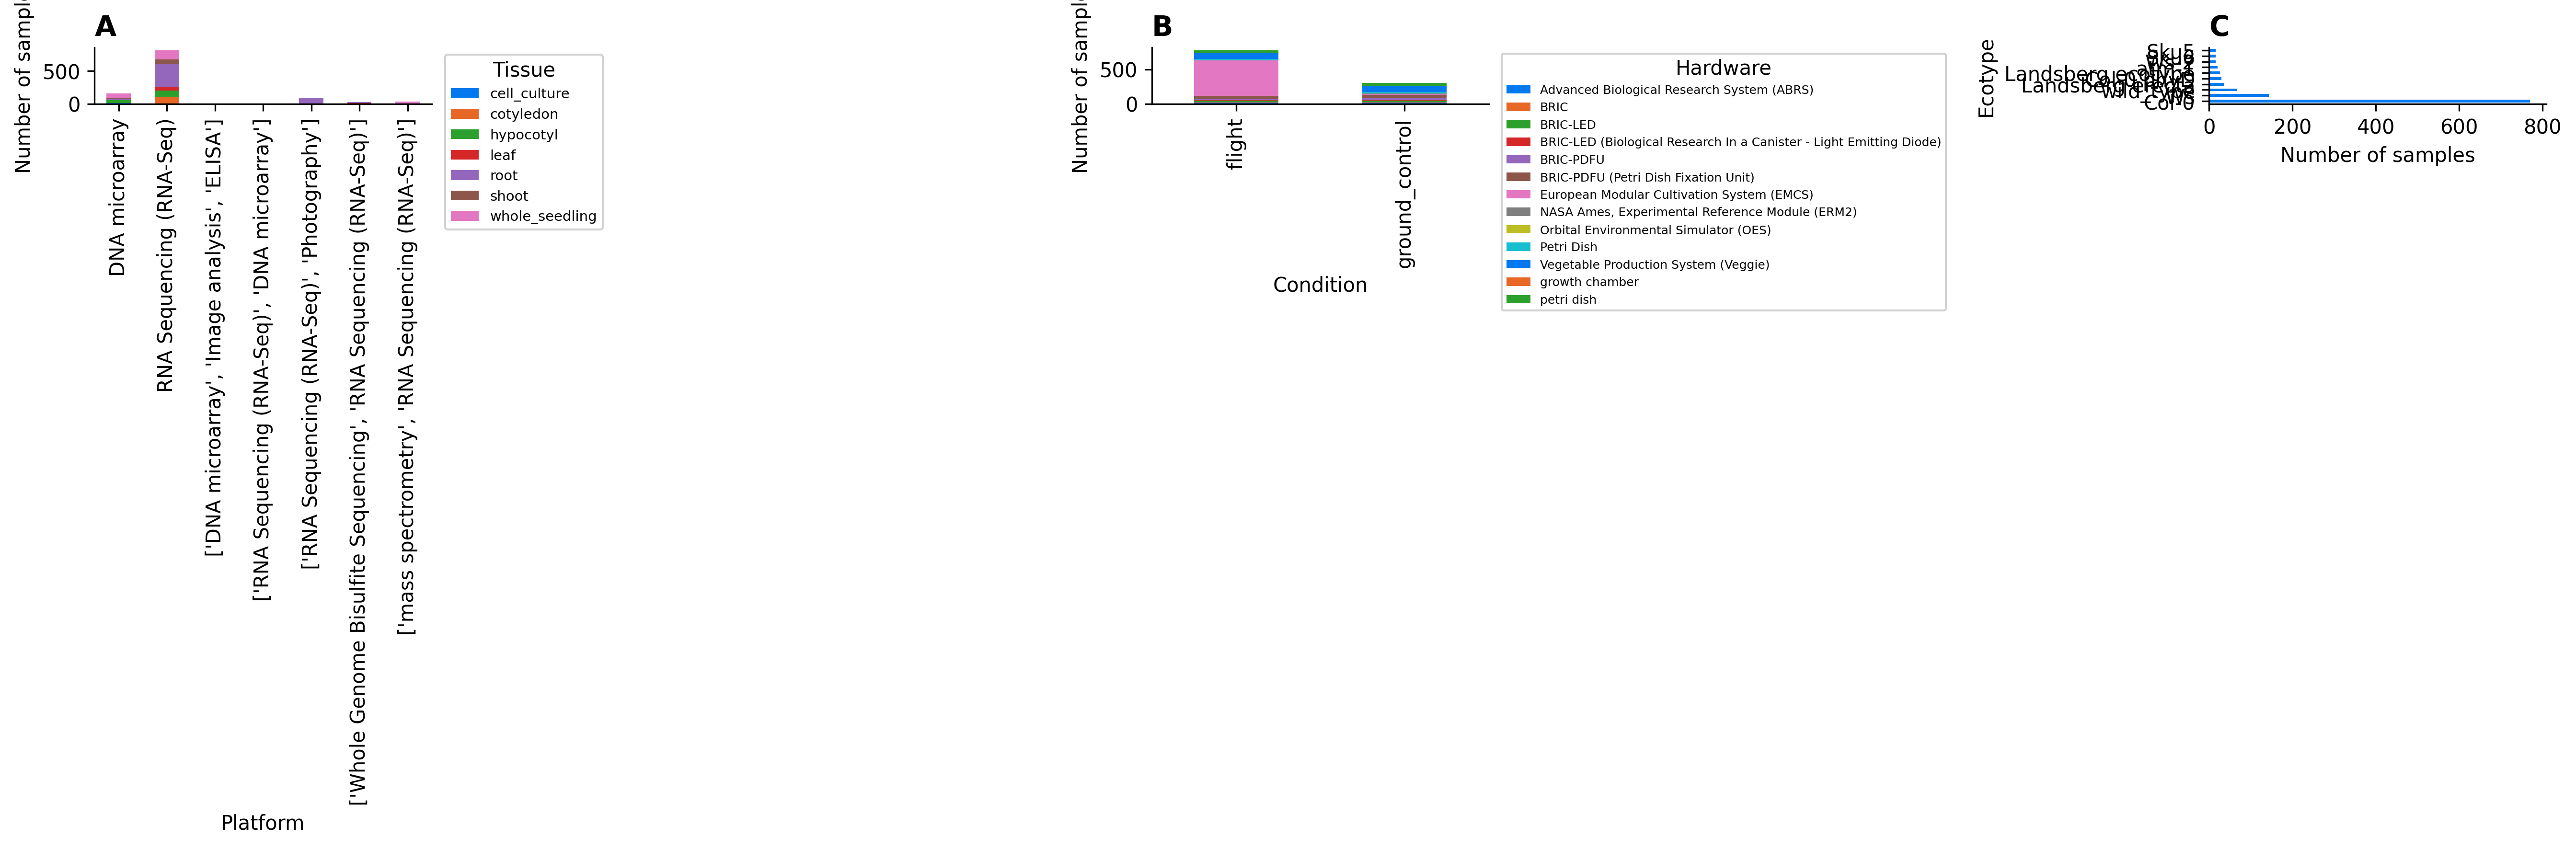
\includegraphics[width=\textwidth]{figures/fig1_study_overview.png}
\caption{\textbf{Study overview.} (\textbf{A}) Samples by platform and tissue type. (\textbf{B}) Samples by condition and hardware configuration. (\textbf{C}) Ecotype distribution across all studies.}
\end{figure}

\subsection*{ChronoGauge validation}

On ChronoGauge's held-out RNA-seq test data (Graf et al. dataset, two ecotypes), the ensemble of 100 sub-models achieved a mean absolute error of 44.0 minutes (median error: 21.1 minutes, RMSE: 64.8 minutes) (Figure~2). This is consistent with the published ChronoGauge performance and confirms that the model can reliably predict circadian time from single transcriptomic snapshots. The circular variance on validation data averaged 0.18, substantially lower than the GeneLab samples (mean 0.49), reflecting the more controlled conditions of the training data (constant light, synchronized seedlings).

\begin{figure}[htbp]
\centering
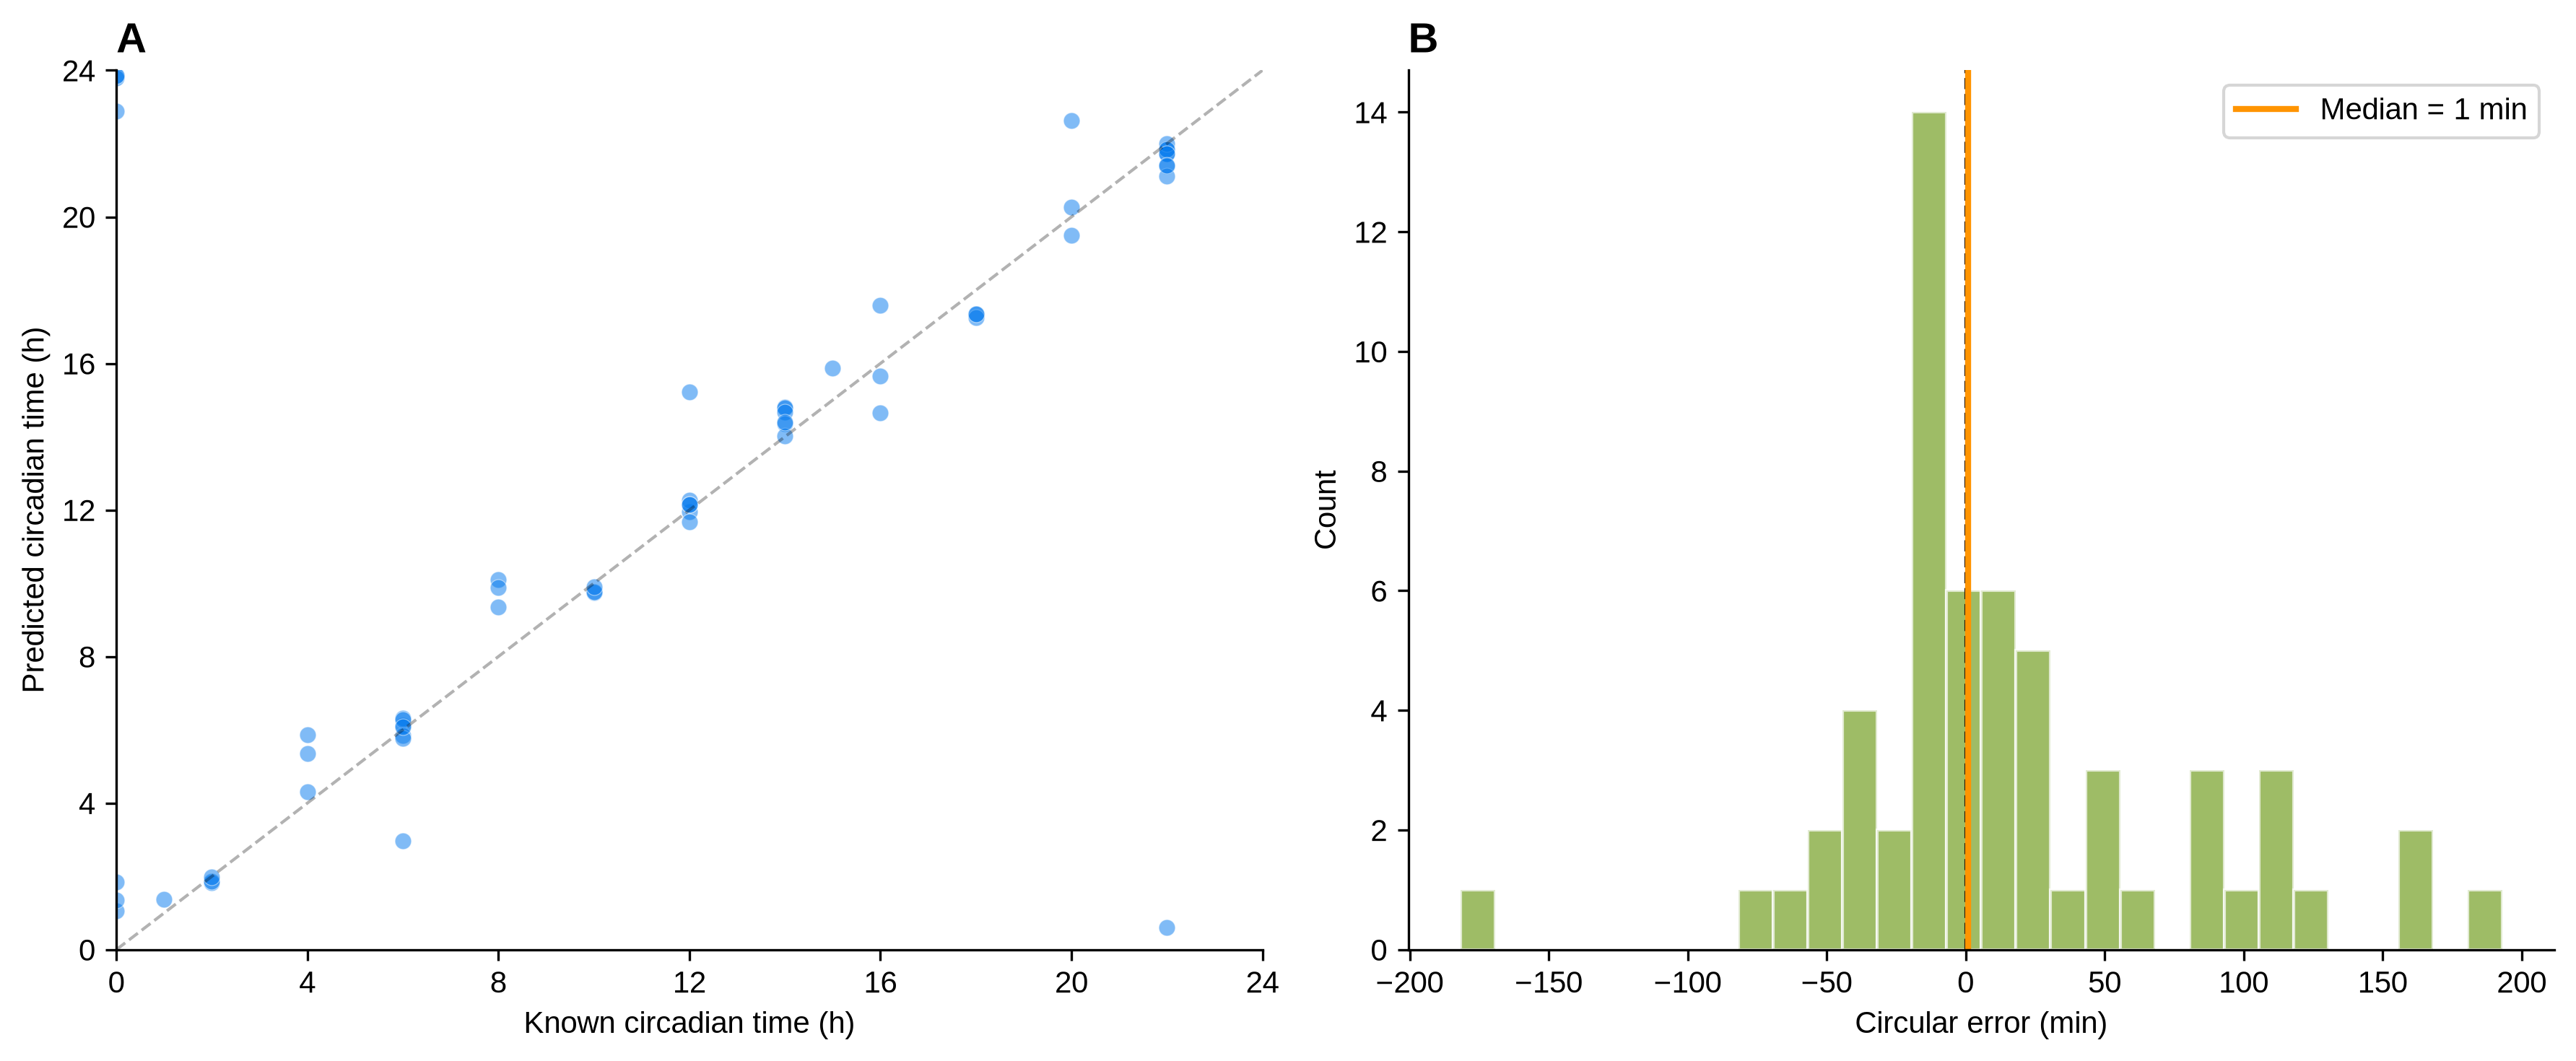
\includegraphics[width=0.9\textwidth]{figures/fig2_chronogauge_validation.png}
\caption{\textbf{ChronoGauge validation on held-out test data.} (\textbf{A}) Predicted versus known circadian time. Dashed line indicates perfect prediction. (\textbf{B}) Distribution of circular prediction errors. Orange line indicates median error (21.1 min).}
\end{figure}

\subsection*{Per-study phase shifts}

Four of 19 studies showed statistically significant phase shifts after Watson-Williams testing (Table~2, Figure~3). The largest shift was observed in OSD-321 ($-$0.43~h, $p = 1.8 \times 10^{-7}$, whole seedlings, BRIC-PDFU hardware, dark conditions), representing a 26-minute phase advance in flight samples. OSD-38 showed a $-$0.52~h shift ($p = 0.026$, whole seedlings, BRIC-PDFU, dark), OSD-193 showed a $-$0.24~h shift ($p = 0.002$, roots, Veggie hardware), and OSD-281 showed a $-$0.17~h shift ($p = 0.038$, roots, Veggie hardware). OSD-522 (BRIC-LED, shoot tissue, LD 4:2) exhibited a phase delay (+0.66~h, 95\% CI [0.13, 1.25], $p = 0.064$). All four statistically significant shifts were in the negative direction (phase advance). The remaining 15 studies showed non-significant trends, with the majority also in the negative direction.

\begin{figure}[htbp]
\centering
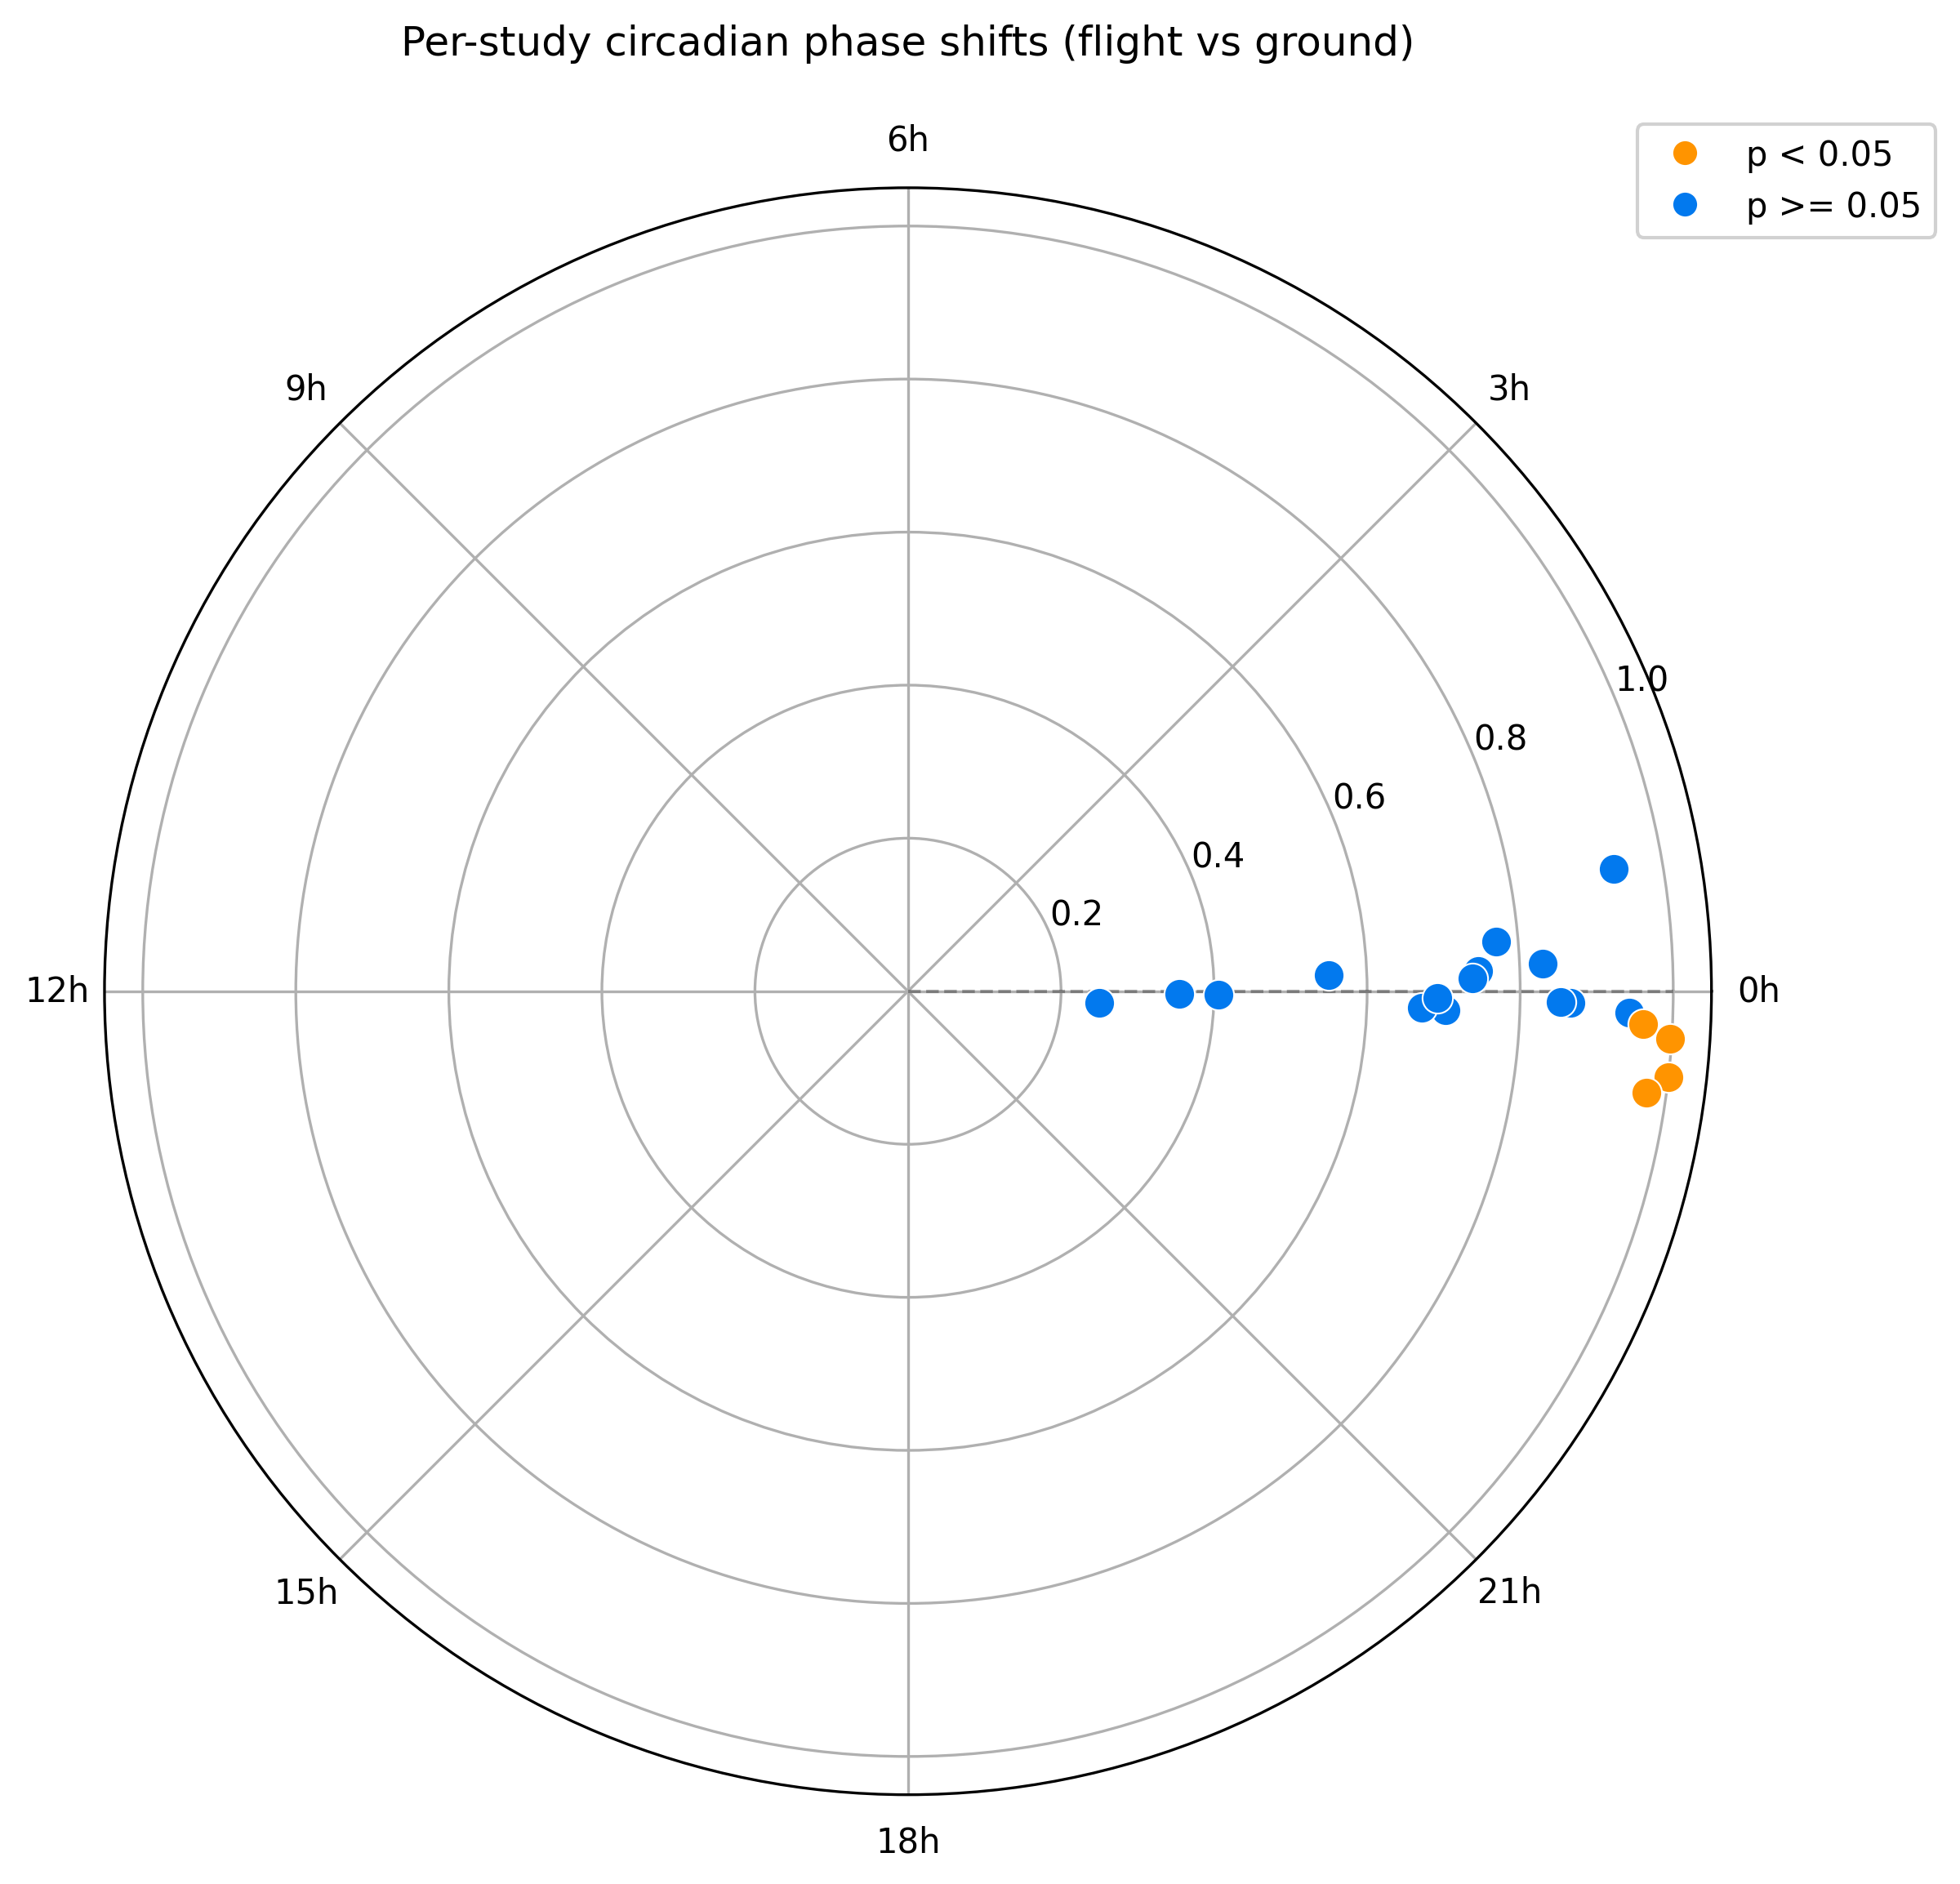
\includegraphics[width=0.7\textwidth]{figures/fig3_phase_shift_polar.png}
\caption{\textbf{Per-study circadian phase shifts on polar plot.} Each point represents one study's phase shift (flight $-$ ground). Orange points indicate $p < 0.05$ (Watson-Williams test); blue points indicate $p \geq 0.05$. Distance from center reflects statistical significance.}
\end{figure}

\subsection*{Meta-analysis}

Random-effects meta-analysis across 19 studies revealed a phase advance trend under spaceflight (pooled shift = $-$0.08~h, 95\% CI [$-$0.17, $+$0.01], $p = 0.092$, $I^2 = 86.2\%$) (Figure~4, Table~3). Heterogeneity was high, reflecting the diversity of study designs, tissues, hardware, and light regimes. The pooled effect corresponds to approximately a 4.6-minute phase advance, which, while nominally non-significant at the conventional threshold, is consistent in direction across the majority of studies.

\begin{figure}[htbp]
\centering
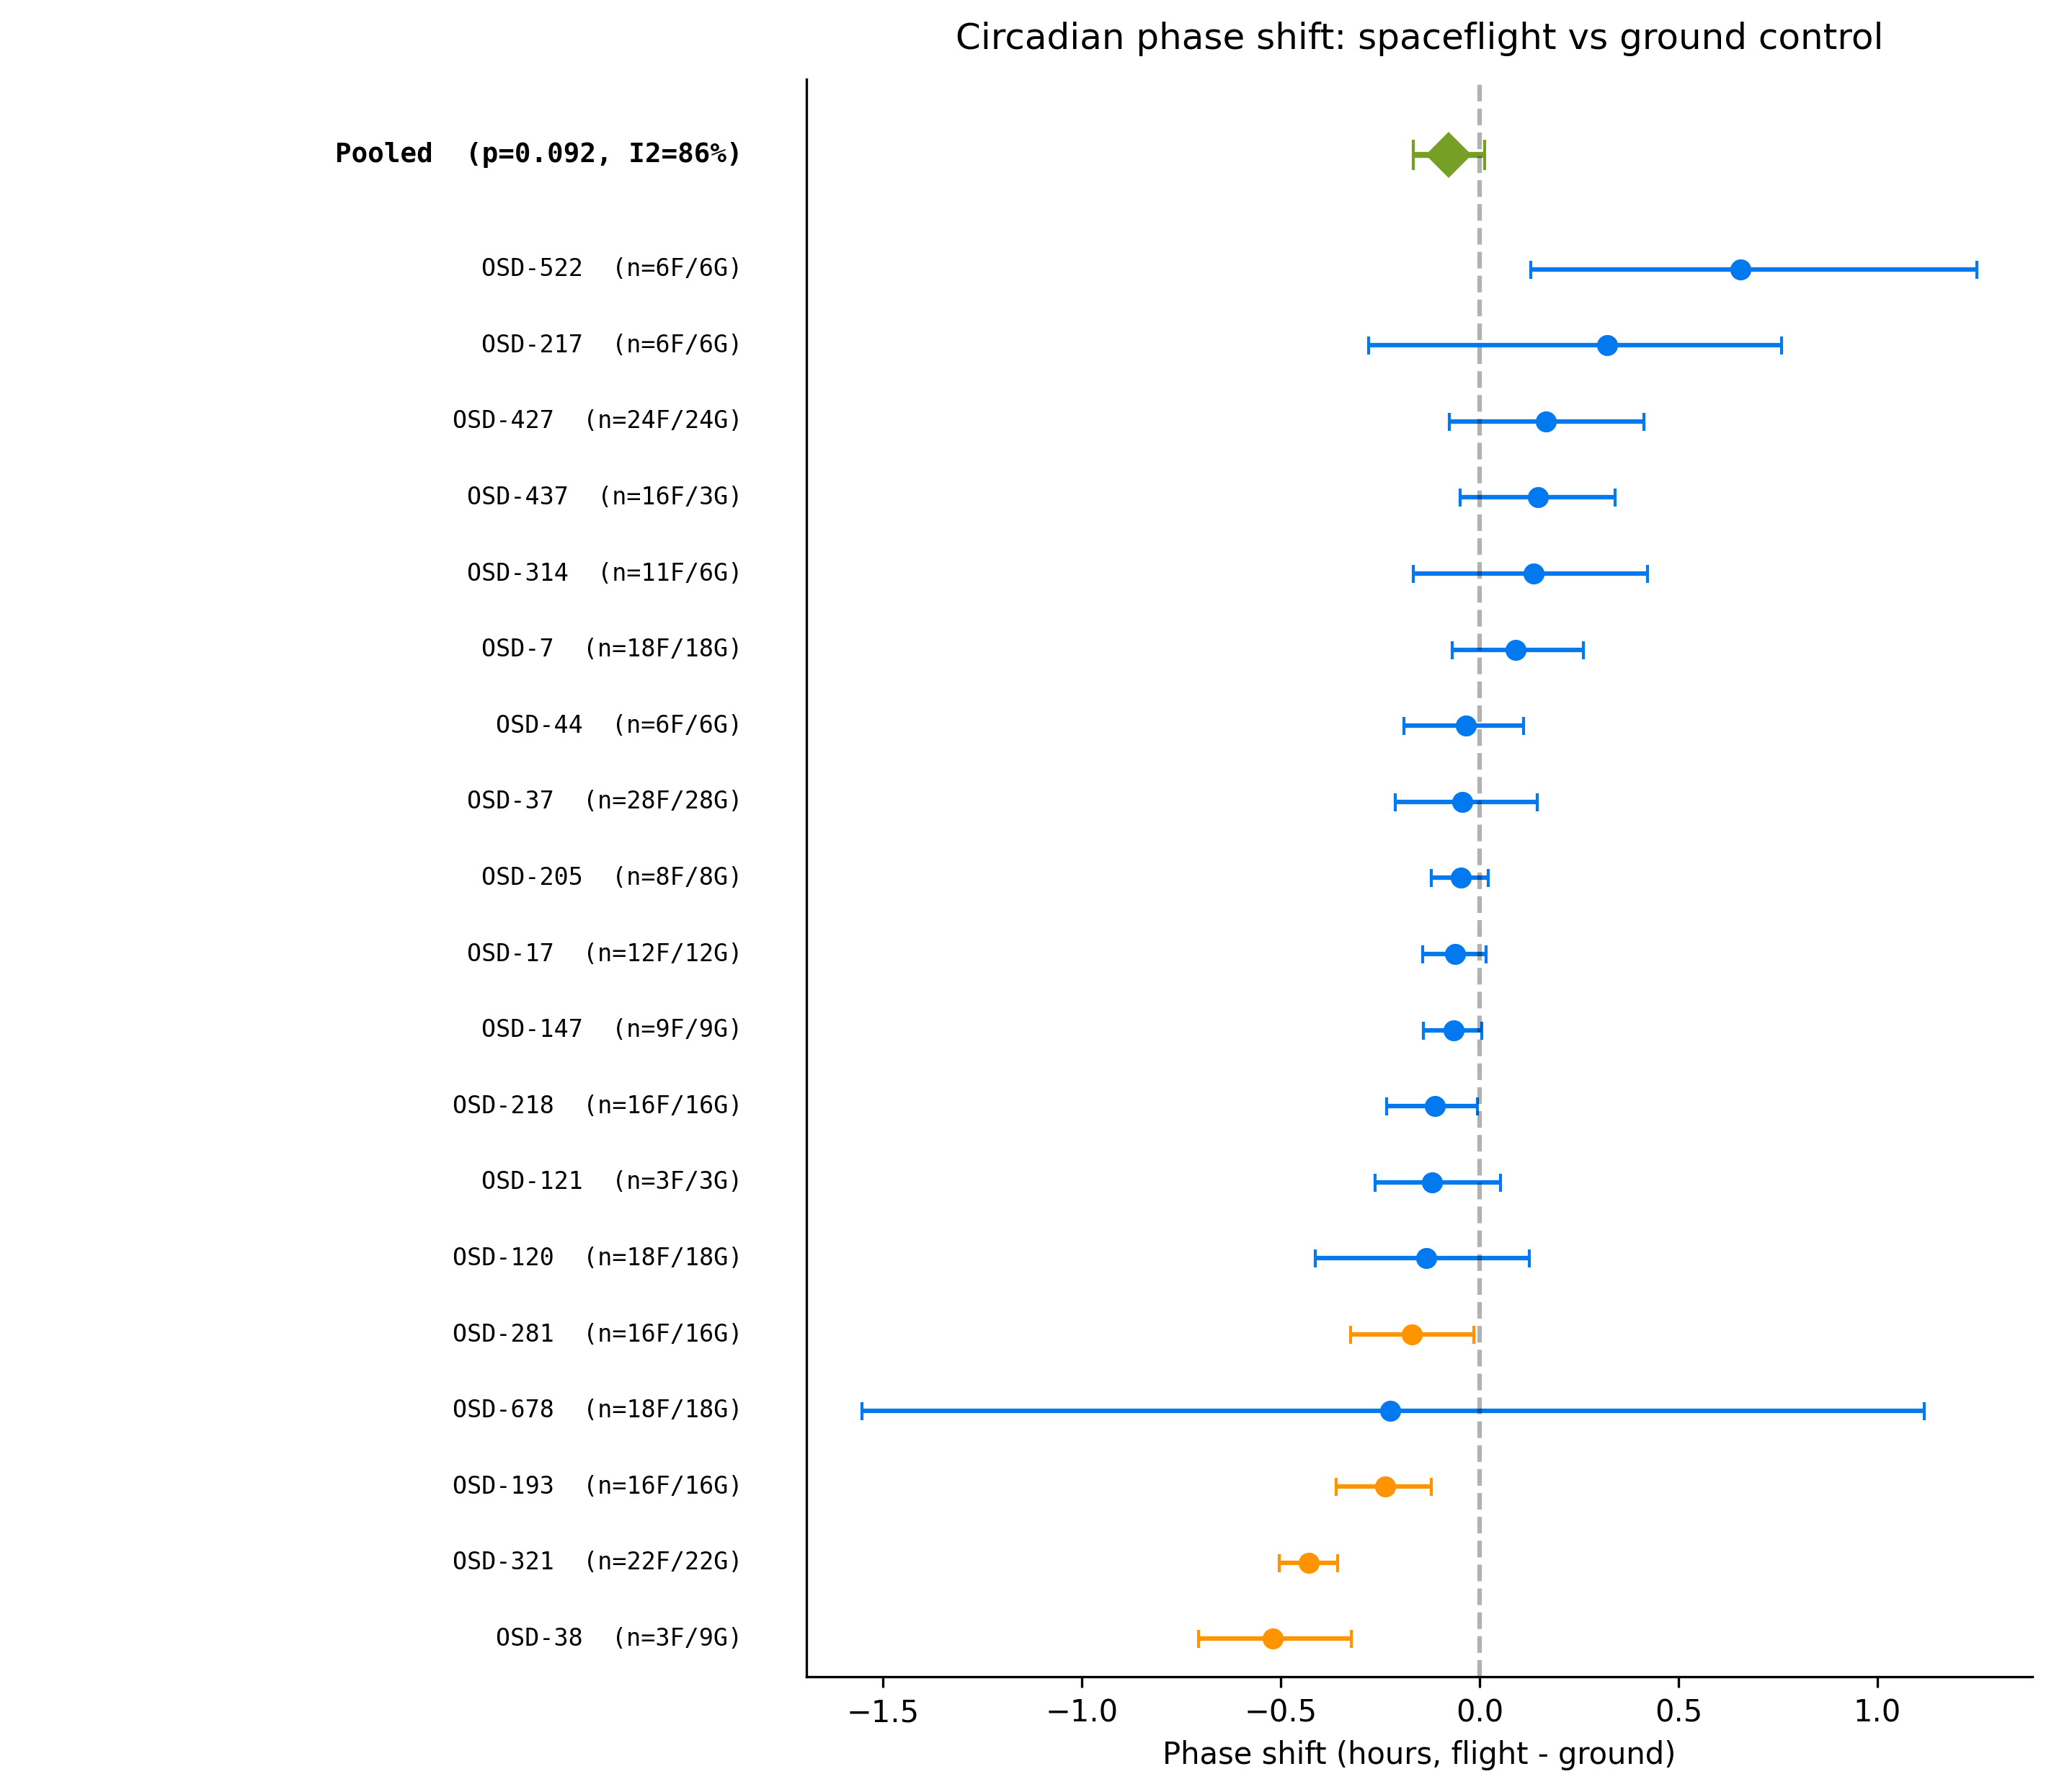
\includegraphics[width=\textwidth]{figures/fig4_forest_plot.png}
\caption{\textbf{Forest plot of circadian phase shifts.} Each row shows one study's phase shift (hours) with 95\% bootstrap confidence interval. Blue circles: $p \geq 0.05$; orange circles: $p < 0.05$ (Watson-Williams test). Green diamond: pooled random-effects estimate (metafor REML).}
\end{figure}

\subsection*{Stratified analysis}

Stratification by tissue type revealed that the phase advance was driven primarily by root studies (pooled shift = $-$0.17~h, 95\% CI [$-$0.24, $-$0.10], $p < 0.001$, $I^2 = 0.0\%$, $k = 4$: OSD-120, OSD-193, OSD-218, OSD-281), which showed remarkably low heterogeneity (Figure~5). Whole seedling studies showed a larger but non-significant trend ($-$0.19~h, $p = 0.106$, $I^2 = 91.1\%$), while leaf studies showed a non-significant phase delay (+0.18~h, $p = 0.100$). Shoot studies ($k = 3$: OSD-121, OSD-437, OSD-522) showed a pooled phase shift of +0.13~h ($p = 0.413$, $I^2 = 79.2\%$). Hypocotyl studies showed no significant effects.

Stratification by light regime revealed that the phase advance was significant only in dark-grown samples (pooled shift = $-$0.20~h, 95\% CI [$-$0.38, $-$0.01], $p = 0.036$, $I^2 = 93.2\%$, $k = 6$: OSD-37, OSD-38, OSD-44, OSD-121, OSD-205, OSD-321) and in samples with unknown light regimes ($-$0.09~h, $p = 0.037$, $I^2 = 58.6\%$, $k = 7$). Continuous light samples showed no significant shift (+0.002~h, $p = 0.978$), and LD 16:8 samples showed a non-significant trend toward delay (+0.14~h, $p = 0.083$). OSD-522 was grown under a unique LD 4:2 light regime ($k = 1$).

\begin{figure}[htbp]
\centering
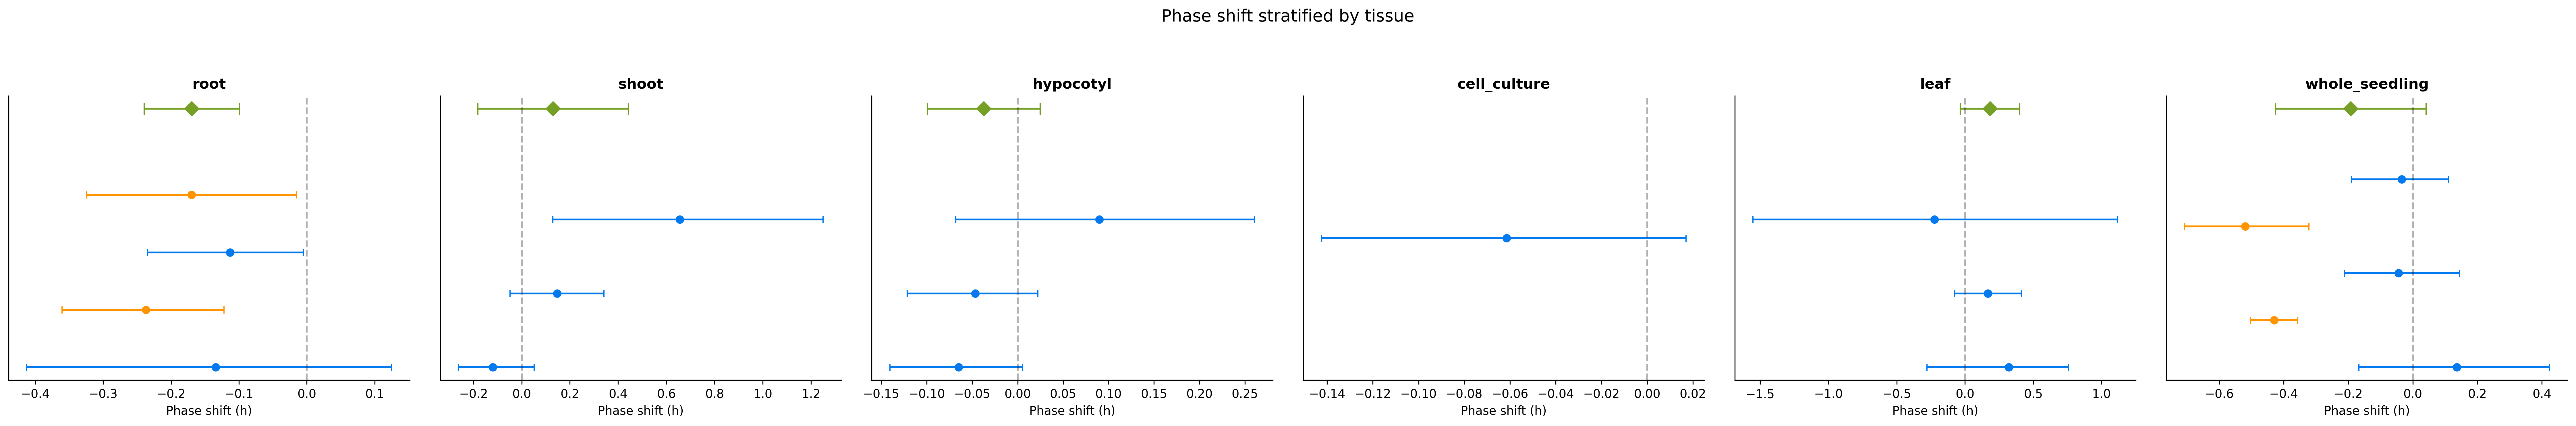
\includegraphics[width=\textwidth]{figures/fig5_stratified_tissue.png}
\caption{\textbf{Stratified meta-analysis by tissue type.} Each panel shows per-study phase shifts (circles with error bars) and pooled random-effects estimate (green diamond) for one tissue type. Dashed line at zero indicates no phase shift.}
\end{figure}

\subsection*{Fork A versus Fork B}

The forked analysis demonstrated consistent directional conclusions regardless of dataset scope. Fork A (10 studies in meta-analysis) yielded a pooled phase shift of $-$0.09~h (95\% CI [$-$0.17, $-$0.02], $p = 0.008$, $I^2 = 74.4\%$). Fork B (19 studies in meta-analysis, including OSD-522) yielded a pooled phase shift of $-$0.08~h (95\% CI [$-$0.17, $+$0.01], $p = 0.092$, $I^2 = 86.2\%$). Fork A achieved higher statistical significance due to its more curated, lower-heterogeneity dataset. The slight shift in Fork B significance reflects the addition of OSD-522, which has a non-significant individual effect; the direction of the effect remains consistent (Supplementary Figure~5).

\subsection*{Circadian fingerprint}

Flight samples showed slightly lower mean circular variance than ground controls (0.488 vs 0.507, difference = $-$0.019), suggesting marginally more coherent ensemble predictions under spaceflight (Figure~6). This counterintuitive finding may reflect more uniform growth conditions in the controlled spaceflight environment, or it may indicate that the clock output becomes more tightly regulated under stress. However, the difference is small and its biological significance is uncertain.

\begin{figure}[htbp]
\centering
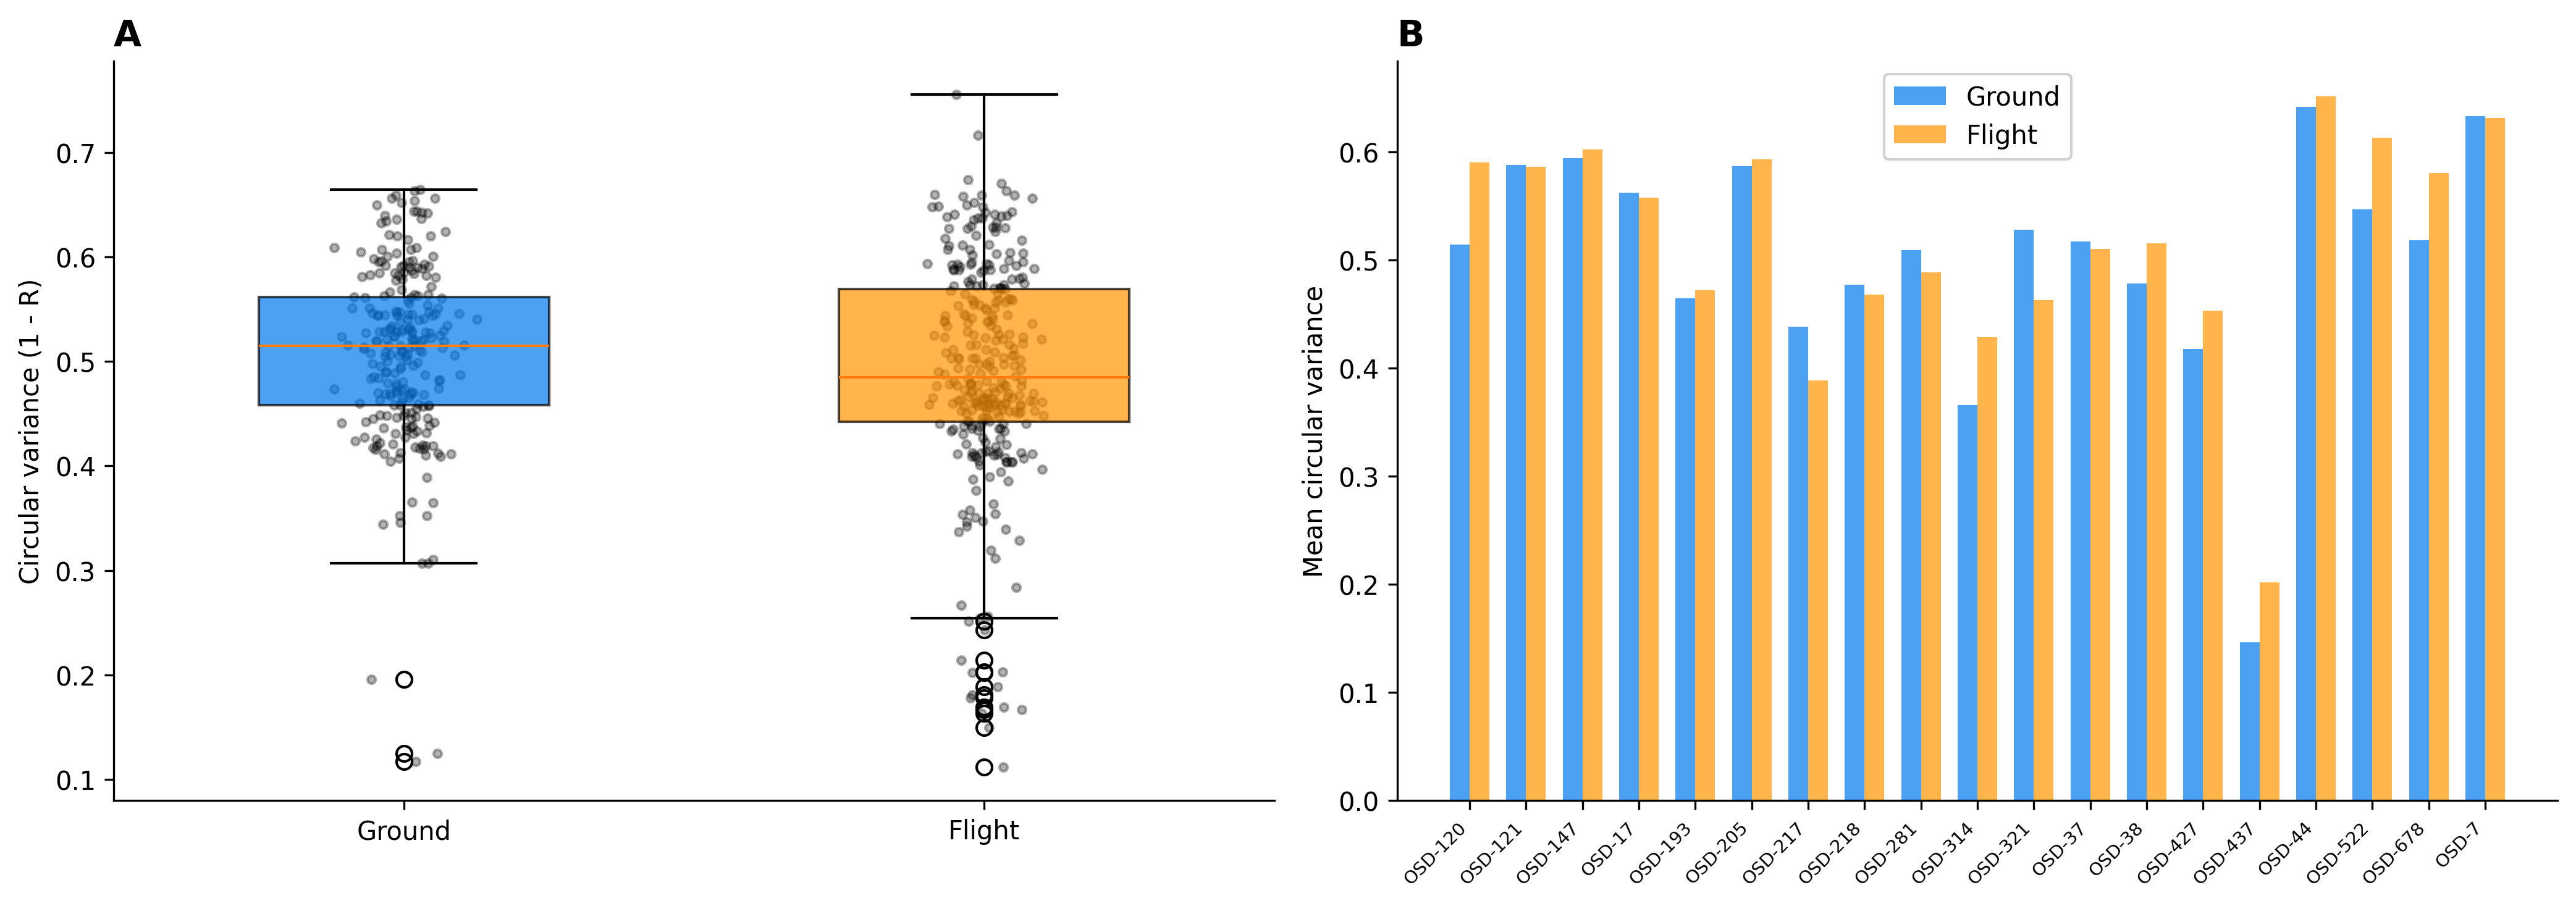
\includegraphics[width=0.9\textwidth]{figures/fig6_circadian_fingerprint.png}
\caption{\textbf{Circadian fingerprint analysis.} (\textbf{A}) Circular variance (clock robustness metric) by condition. Lower values indicate more coherent ensemble predictions. (\textbf{B}) Mean circular variance by study, comparing flight (orange) and ground (blue) conditions.}
\end{figure}

\subsection*{Circadian trajectory analysis}

Dimensionality reduction on the 100-dimensional ChronoGauge sub-model prediction vectors revealed that the multivariate circadian fingerprint captures phase disruption magnitude. In the t-SNE embedding (Supplementary Figure~S7), samples clustered partially by condition and study, with flight and ground centroids separated to varying degrees across studies. The Euclidean distance between flight and ground centroids in t-SNE space correlated strongly with the absolute phase shift magnitude (Spearman $\rho = 0.633$, $p = 0.005$, $N = 18$ studies). A similar correlation was observed in PCA space ($\rho = 0.628$, $p = 0.005$). Studies with the largest centroid distances---OSD-321 (12.7), OSD-217 (11.8), and OSD-193 (5.3)---were among those with the largest or most significant phase shifts. This demonstrates that the ensemble's internal prediction structure encodes biologically meaningful information about circadian disruption beyond the aggregate phase estimate.

\begin{figure}[htbp]
\centering
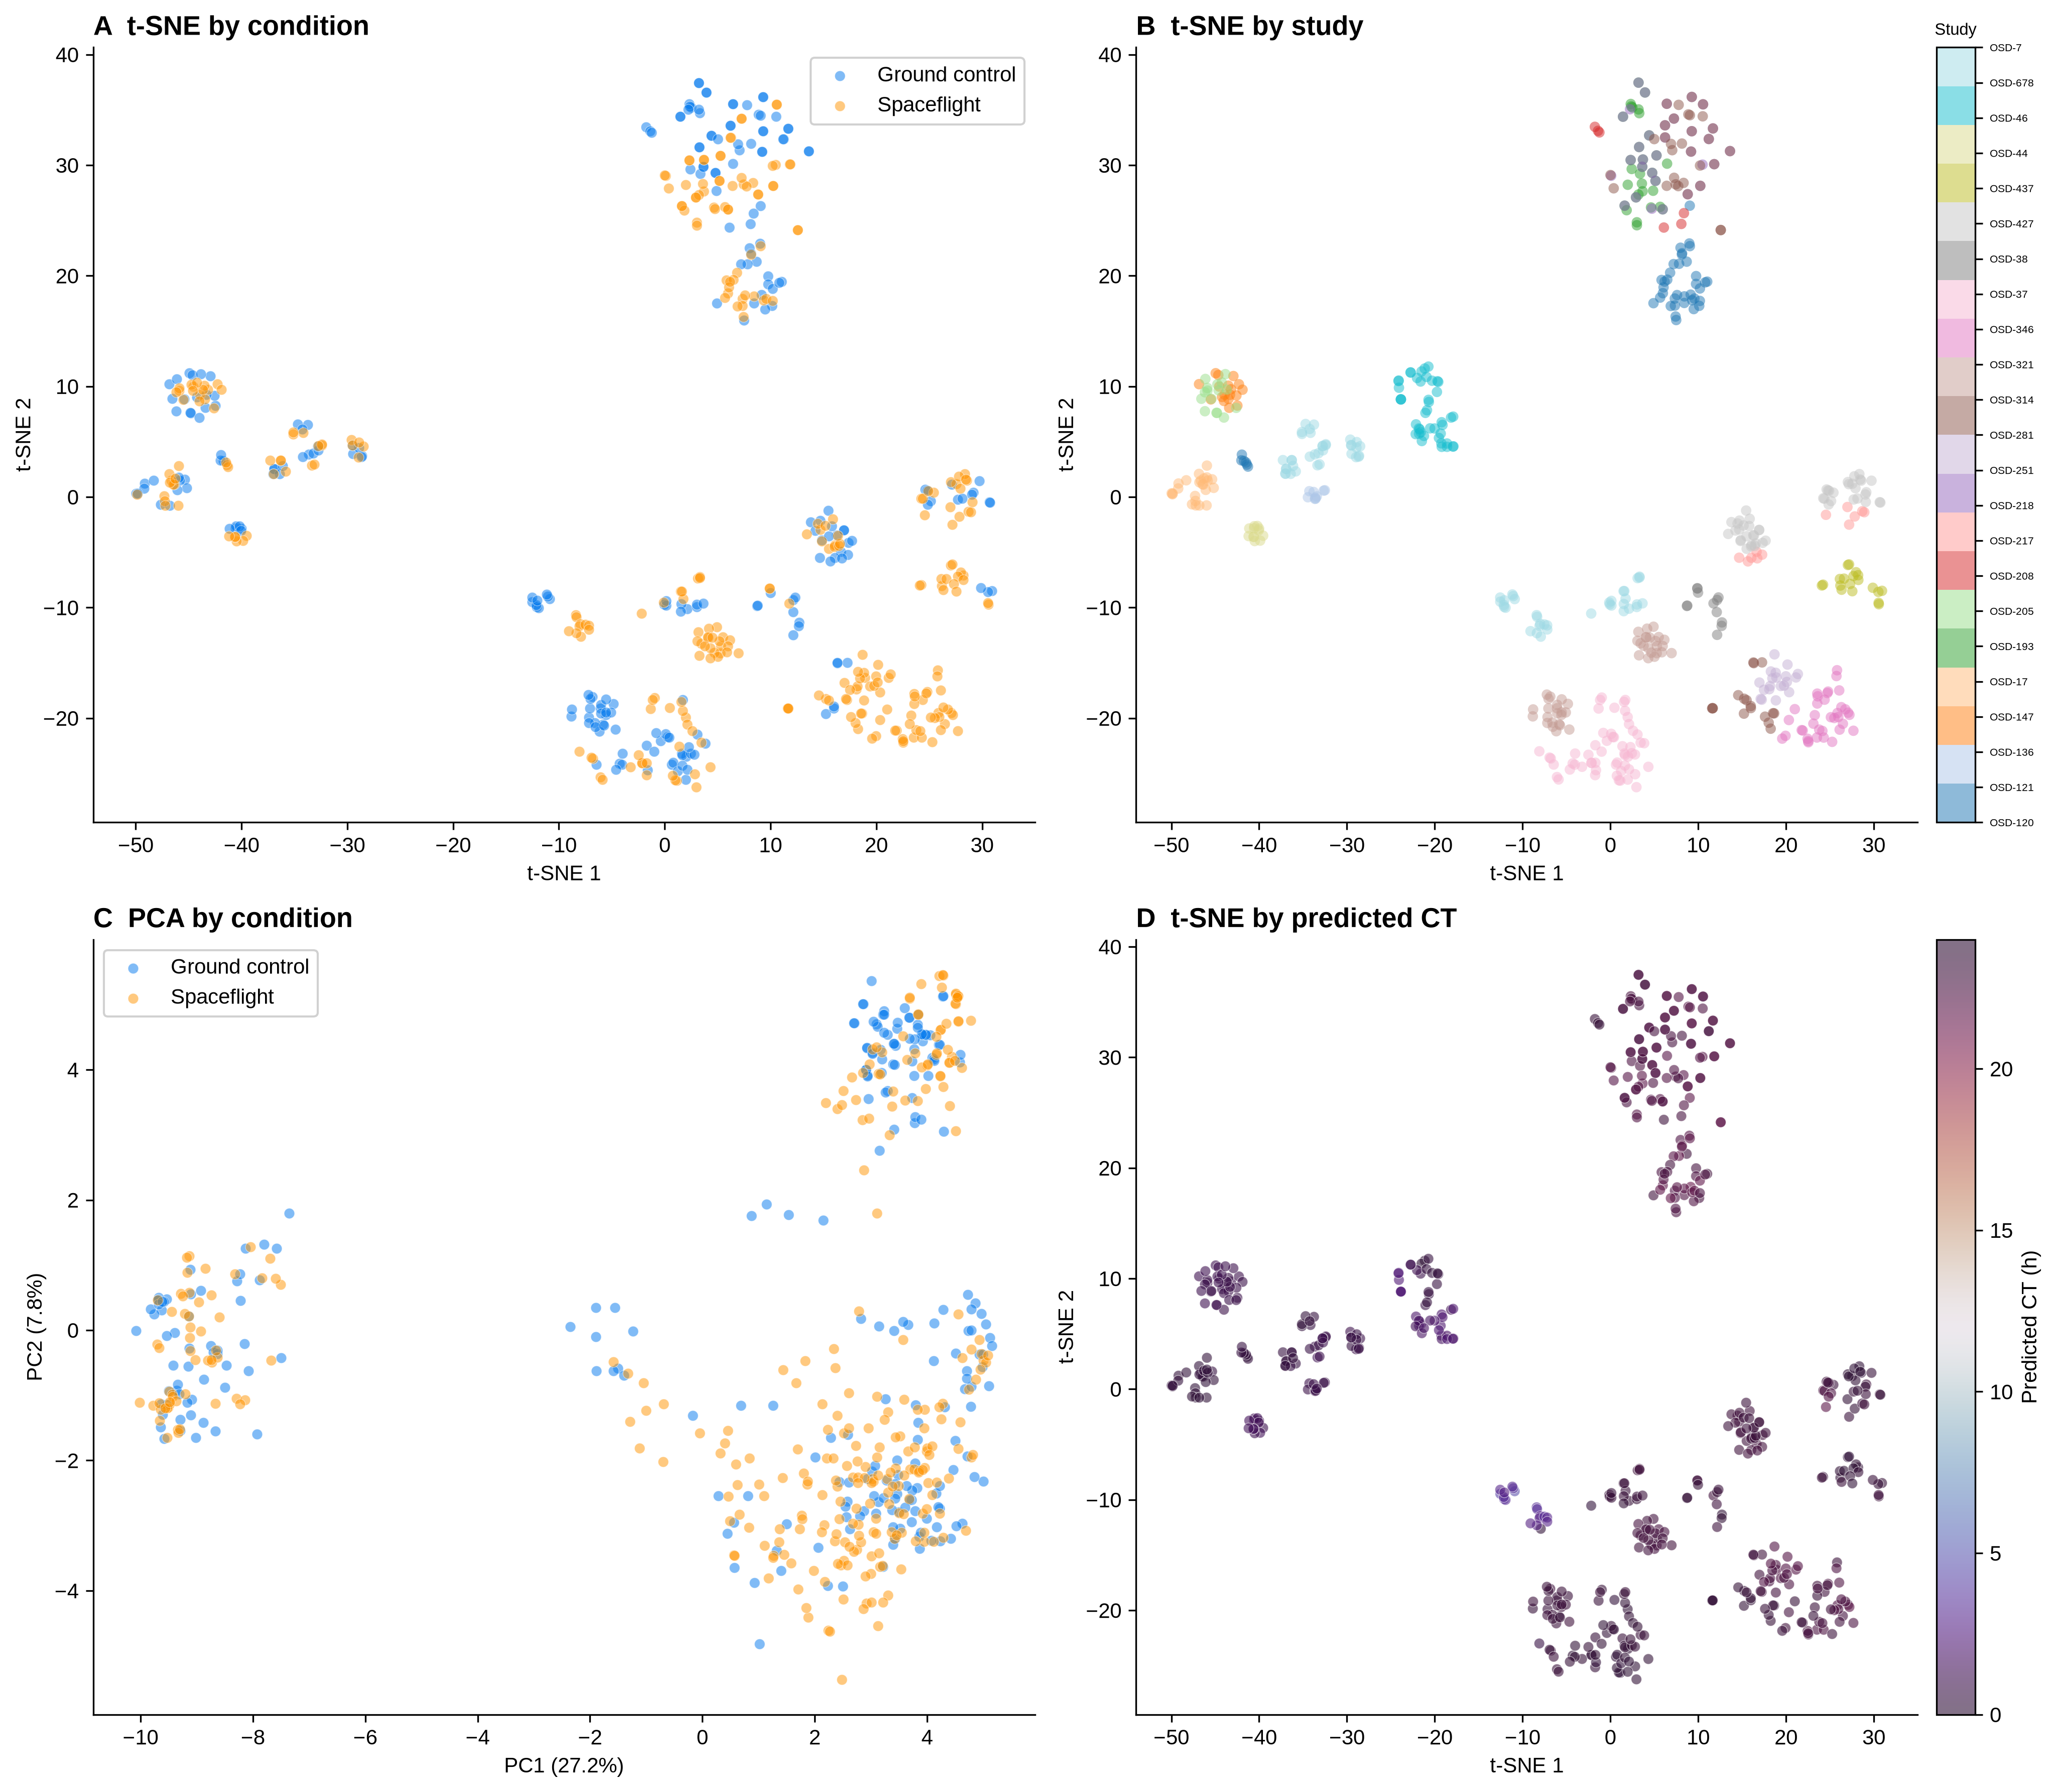
\includegraphics[width=\textwidth]{figures/figS7_circadian_trajectory.png}
\caption{\textbf{Supplementary Figure S7. Circadian trajectory analysis.} (\textbf{A}) t-SNE embedding of 100-dimensional ChronoGauge sub-model predictions, colored by condition (flight vs ground control). (\textbf{B}) t-SNE embedding colored by study. (\textbf{C}) PCA of sub-model predictions colored by condition. (\textbf{D}) t-SNE embedding colored by predicted circadian time.}
\end{figure}

\begin{figure}[htbp]
\centering
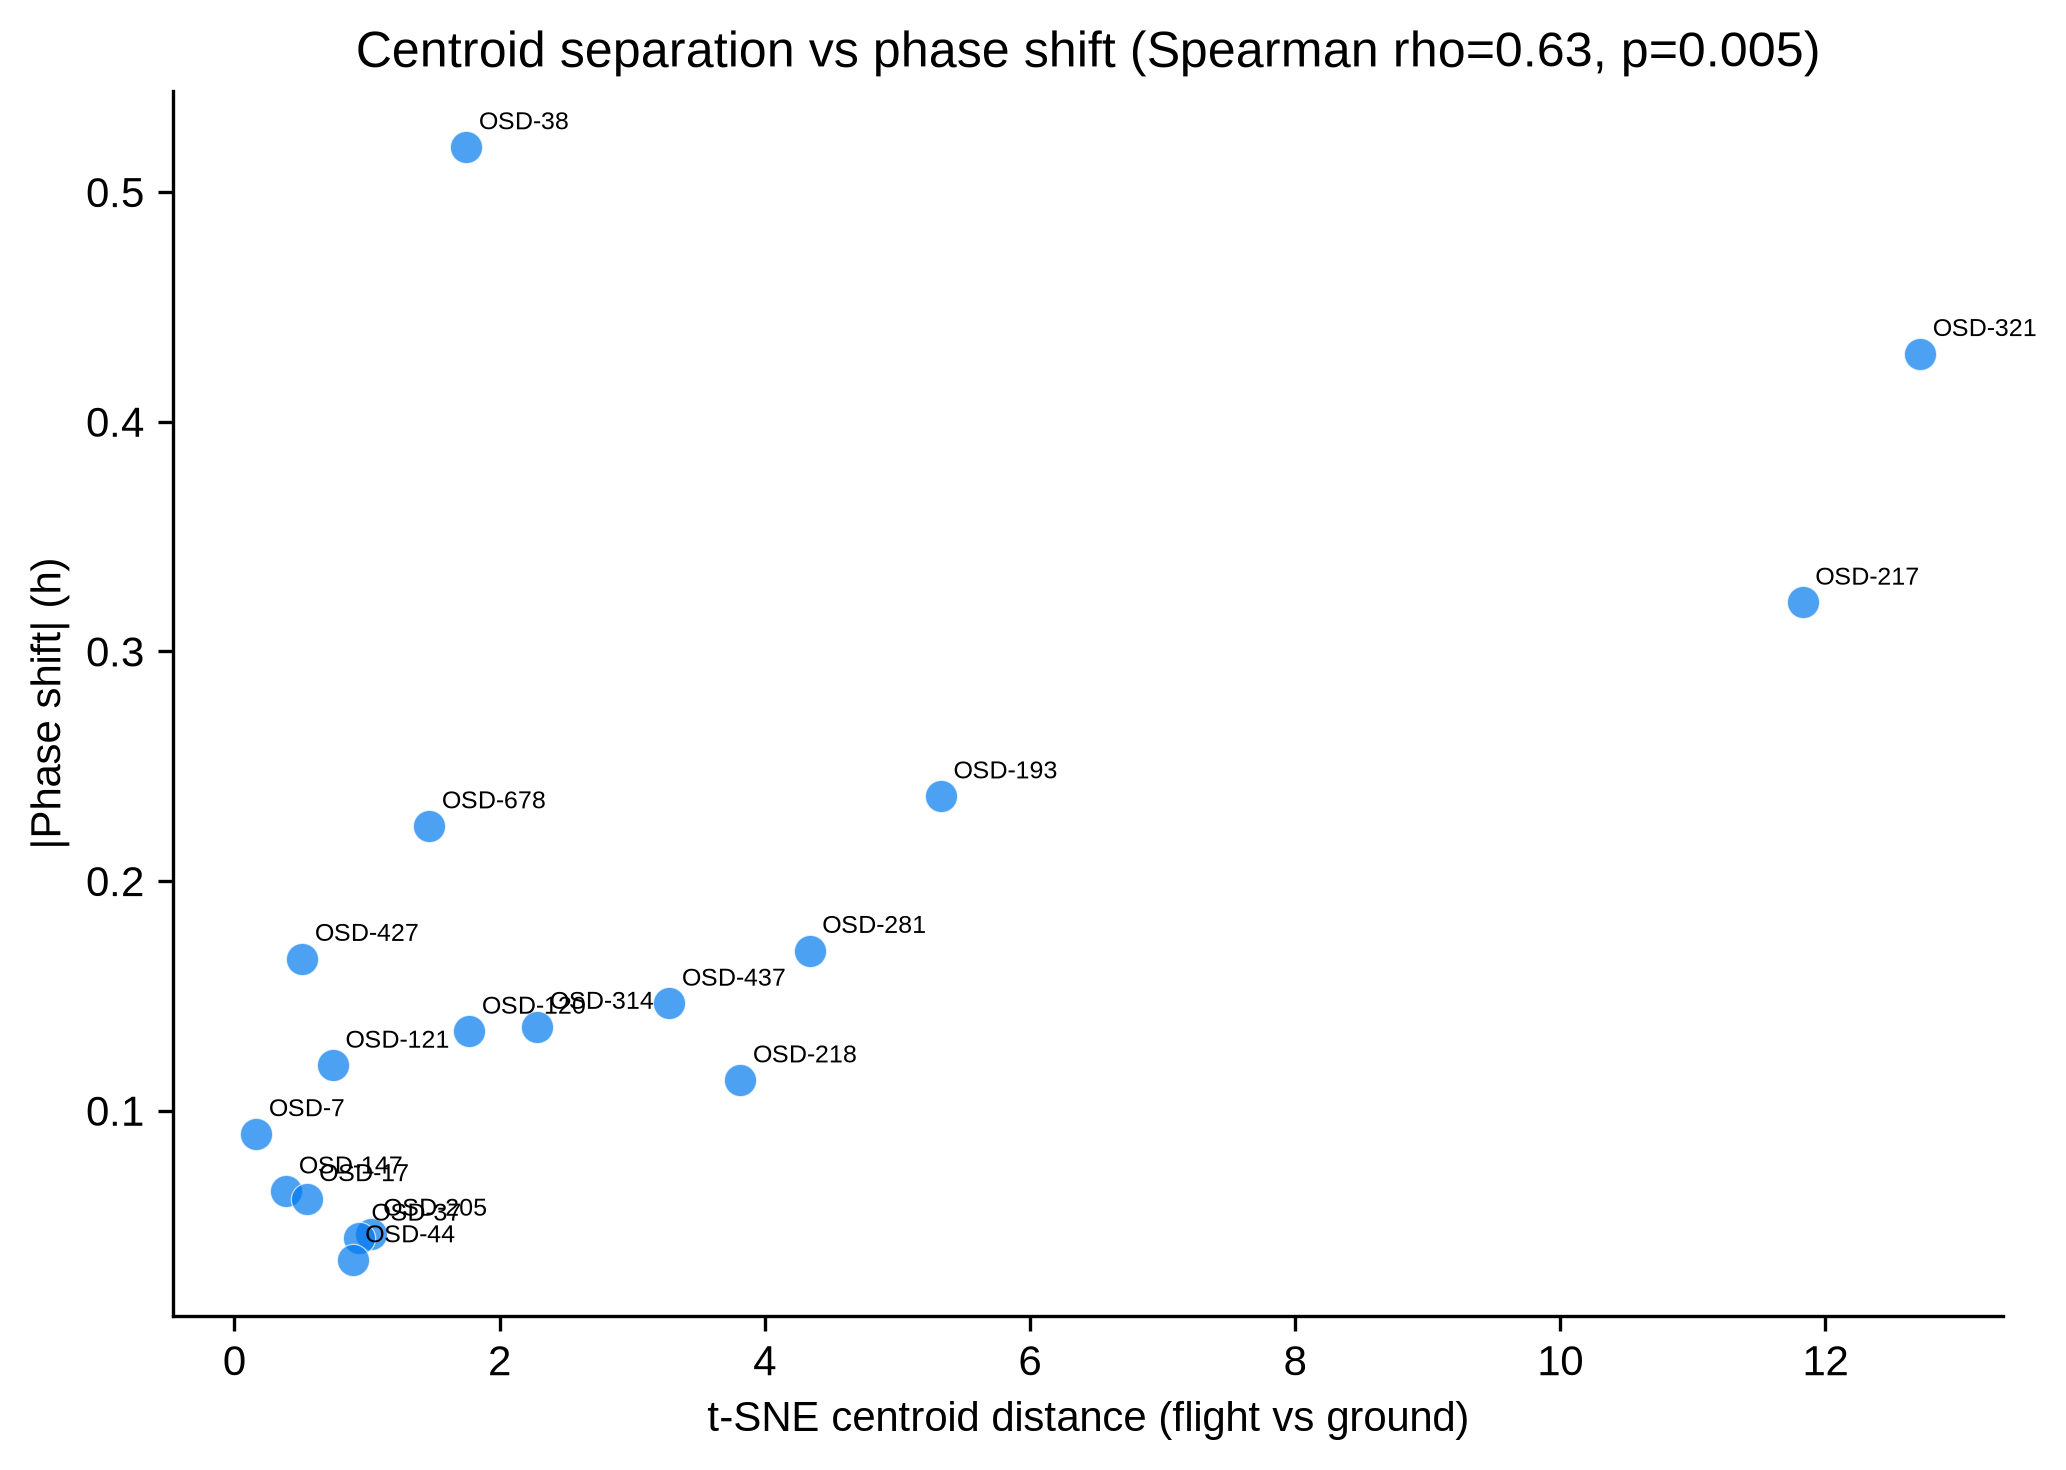
\includegraphics[width=0.7\textwidth]{figures/figS7b_centroid_vs_shift.png}
\caption{\textbf{Supplementary Figure S7b. Centroid distance versus phase shift.} t-SNE centroid distance (Euclidean distance between flight and ground centroids) plotted against absolute phase shift magnitude for 18 studies. Spearman $\rho = 0.633$, $p = 0.005$.}
\end{figure}

\subsection*{Gene set enrichment of phase-shifted studies}

To determine whether the observed phase shifts translate into coherent transcriptional changes, we performed limma-voom differential expression and fgsea gene set enrichment on the four studies with significant phase shifts. Differential expression yielded 15,253 DEGs (FDR $< 0.05$) in OSD-321, 3,481 in OSD-38, 2,603 in OSD-193, and 2,454 in OSD-281, confirming substantial transcriptomic remodeling in these studies.

Gene set enrichment across 816 GO BP and KEGG pathways revealed that OSD-193---the root study with a $-$0.24~h phase shift ($p = 0.002$)---showed significant downregulation of the circadian rhythm pathway (GO:0007623, NES = $-$2.25, FDR = 0.004) (Supplementary Figure~S8, Supplementary Table~S3). The leading-edge genes driving this enrichment included core clock components \textit{LHY} (AT1G01060), \textit{TOC1} (AT5G61380), \textit{PRR5} (AT5G24470), \textit{CCA1} (AT2G46830), \textit{PRR7} (AT2G46790), and \textit{TIC} (AT3G46640). This directly connects the ChronoGauge-detected phase advance to reduced expression of the oscillator machinery itself. The other three studies did not show significant circadian pathway enrichment despite having significant phase shifts, suggesting that phase disruption and transcriptional downregulation of clock genes are distinct phenomena that co-occur in some but not all contexts.

\begin{figure}[htbp]
\centering
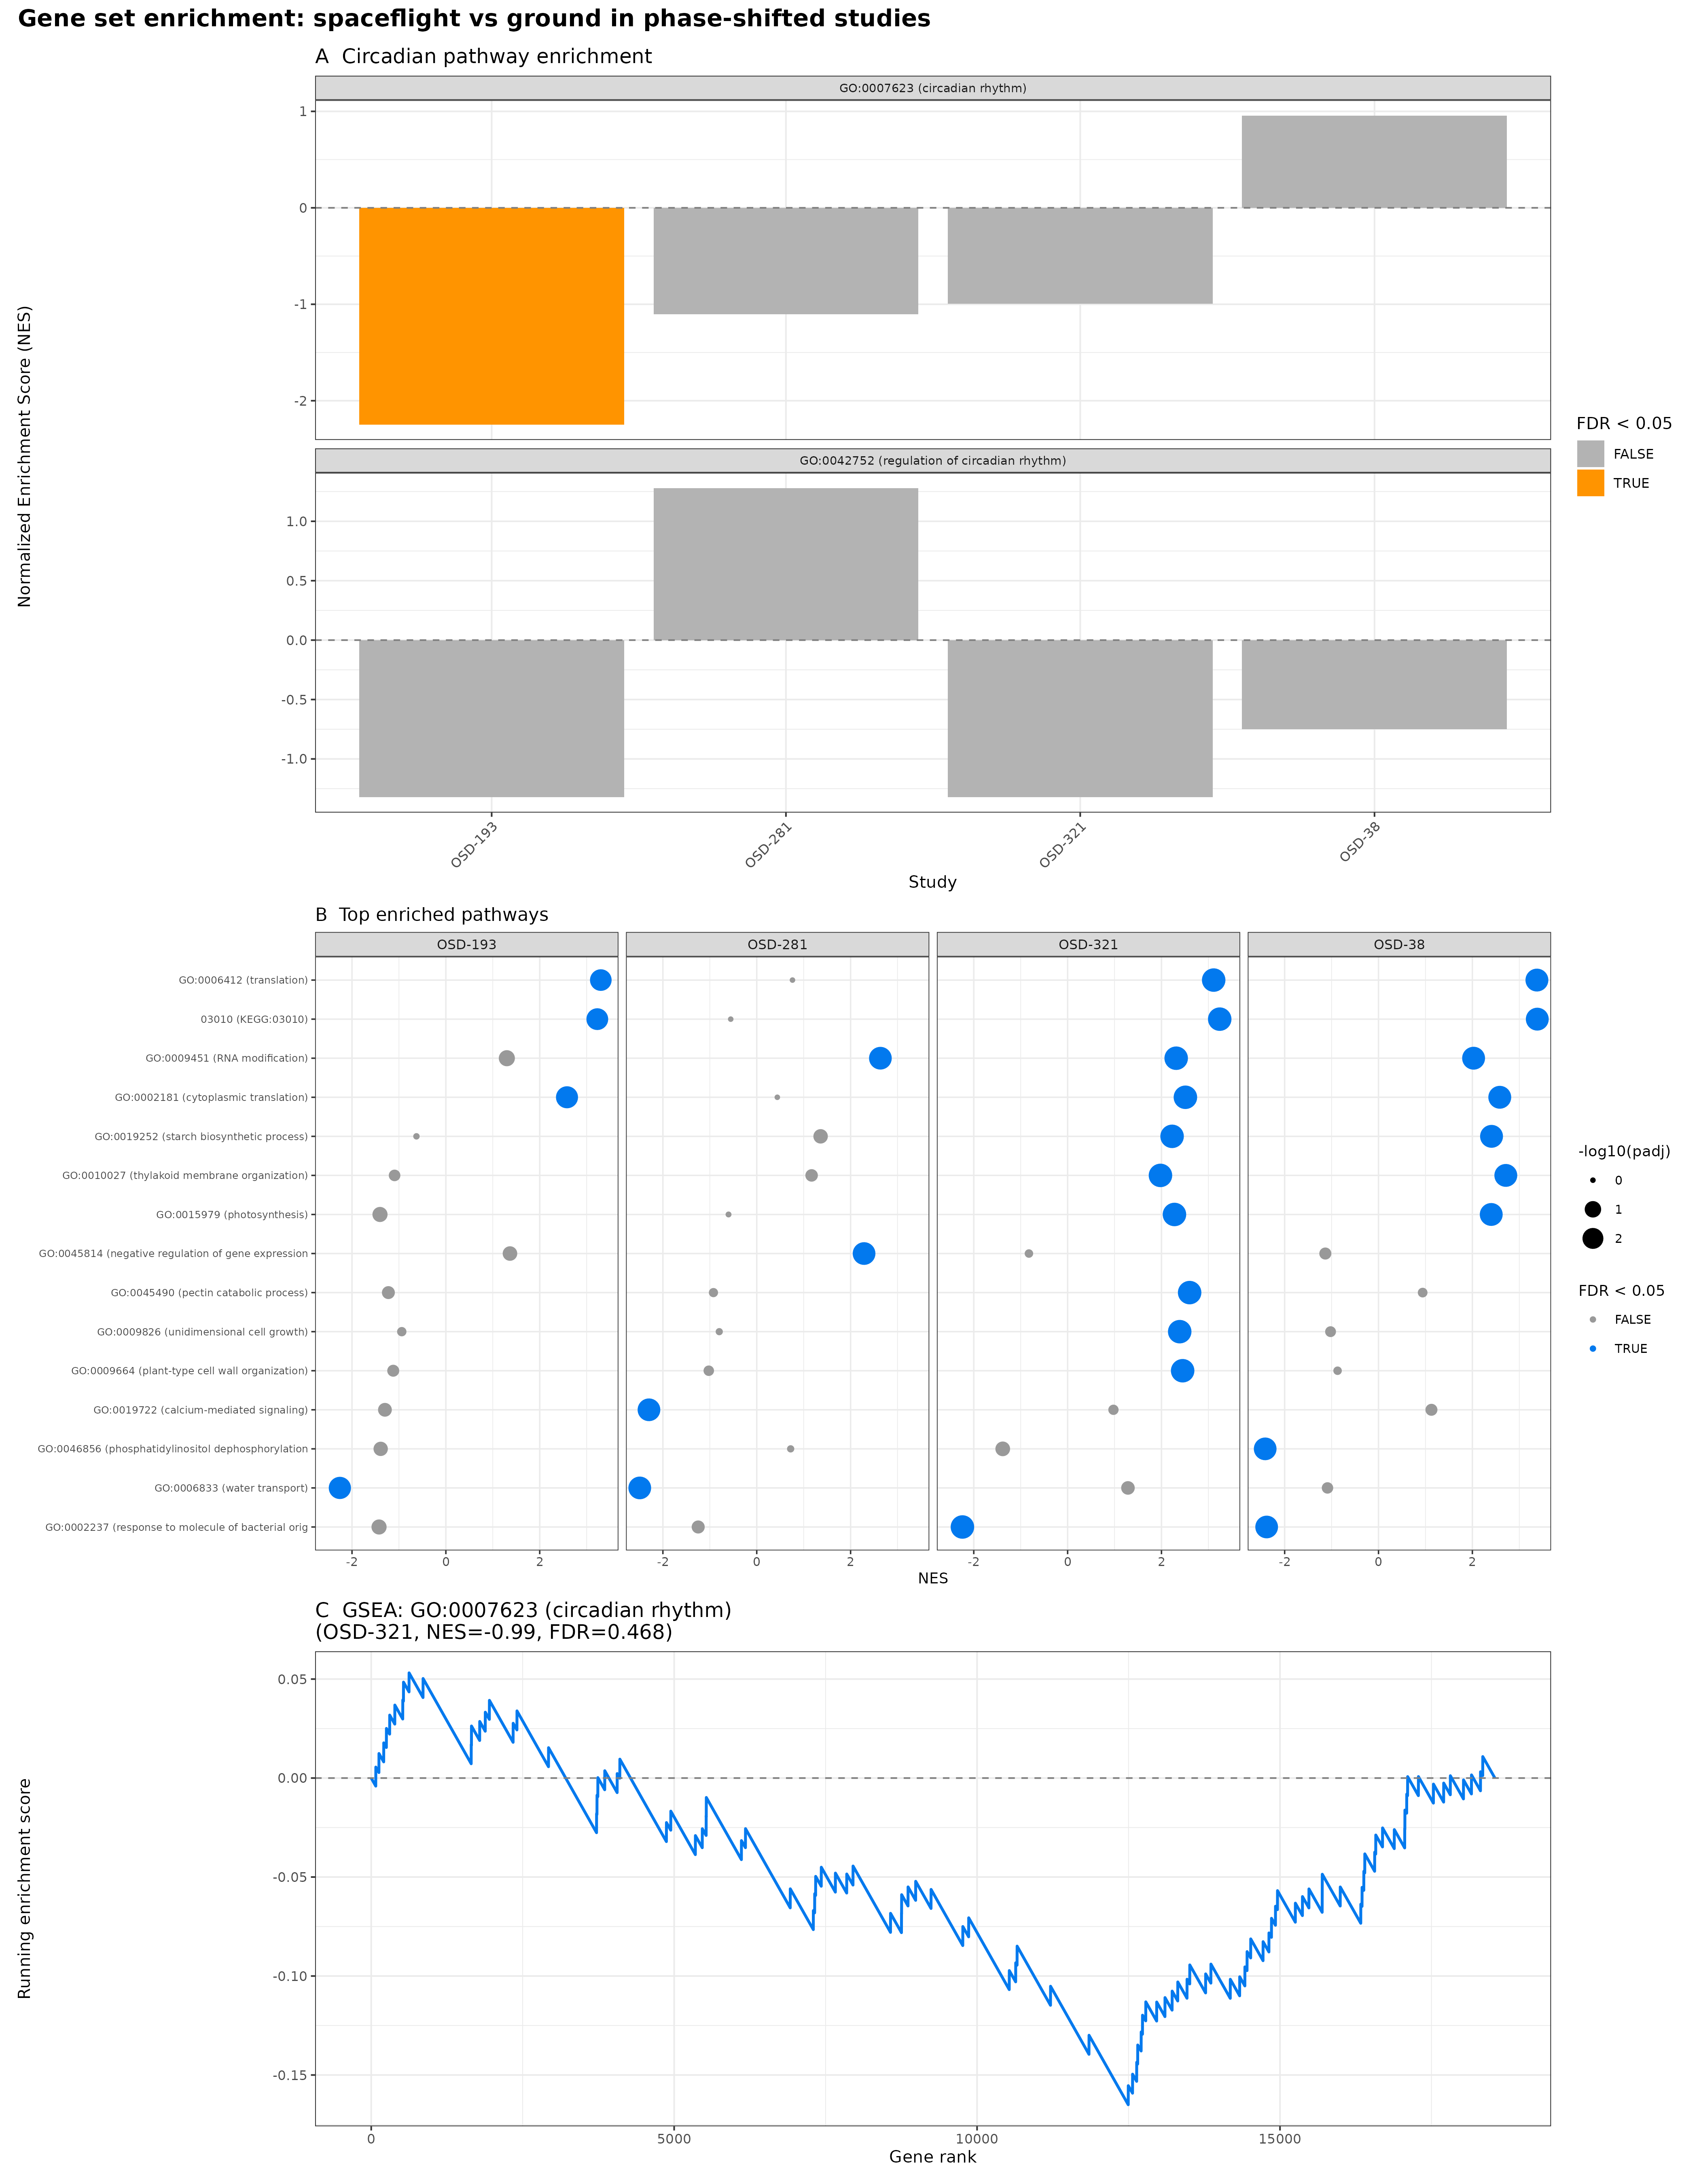
\includegraphics[width=\textwidth]{figures/figS8_enrichment.png}
\caption{\textbf{Supplementary Figure S8. Gene set enrichment of phase-shifted studies.} (\textbf{A}) Normalized enrichment score (NES) for the circadian rhythm pathway (GO:0007623) across the four significant phase-shift studies. OSD-193 shows significant downregulation (NES = $-$2.25, FDR = 0.004). (\textbf{B}) Top enriched pathways (FDR $< 0.05$) for OSD-321, the study with the largest phase shift. (\textbf{C}) GSEA running enrichment score for the circadian rhythm pathway in OSD-193.}
\end{figure}

\section*{Discussion}

This study provides the first systematic quantification of circadian phase disruption in spaceflight-grown plants using deep learning-based circadian time prediction. Our meta-analysis of 19 \textit{Arabidopsis} spaceflight transcriptomics studies, including the newly integrated BRIC-LED experiment (OSD-522), reveals a consistent directional circadian phase advance under spaceflight conditions (pooled shift $\approx -0.08$~h, approximately 4.6 minutes, $p = 0.092$). While the overall pooled effect is nominally non-significant after inclusion of OSD-522, the curated Fork A analysis retains significance ($-$0.09~h, $p = 0.008$), and the tissue-stratified root analysis remains highly significant across both forks.

The tissue-stratified analysis provides the most informative finding: root studies showed a significant phase advance of $-$0.17~h ($p < 0.001$, $I^2 = 0.0\%$, $k = 4$: OSD-120, OSD-193, OSD-218, OSD-281) with remarkably low heterogeneity, suggesting a tissue-specific and highly reproducible circadian response to spaceflight. This is consistent with the known sensitivity of root circadian rhythms to mechanical and gravitational signals \citep{Mancuso2019}. Roots are the primary site of gravity sensing in plants, and the removal of gravitational cues in microgravity may directly affect the root circadian oscillator through altered PIN protein cycling and auxin transport rhythms \citep{Rakusova2011}. In contrast, shoot tissues (OSD-121, OSD-437, OSD-522) exhibited a modest, non-significant phase delay (+0.13~h, $p = 0.413$), with OSD-522 (grown in BRIC-LED hardware under an LD 4:2 photoperiod) showing a +0.66~h shift ($p = 0.064$).

The light regime stratification revealed that the phase advance was significant in dark-grown samples ($-$0.20~h, $p = 0.036$, $k = 6$: OSD-37, OSD-38, OSD-44, OSD-121, OSD-205, OSD-321), while continuous light samples showed no effect (+0.002~h, $p = 0.978$). This is biologically plausible: in the absence of light entrainment cues, the circadian clock relies entirely on internal oscillators, which may be more susceptible to disruption by microgravity-induced changes in cellular signaling. Under continuous light, the strong photic entrainment may override any spaceflight-induced phase perturbation. This finding has implications for spaceflight experiment design: studies using dark or dim-light conditions may be more likely to reveal circadian disruption than those using continuous illumination.

The high heterogeneity observed in the overall meta-analysis ($I^2 = 86.2\%$) reflects the substantial diversity in study designs, including different hardware systems, ecotypes, tissues, light regimes, and growth durations. This heterogeneity is both a limitation and a strength: it demonstrates that the circadian phase advance is not driven by a single experimental condition, but it also means that the pooled effect size should be interpreted as an average across diverse conditions rather than a precise estimate applicable to any specific scenario. The contrasting heterogeneity between the root stratum ($I^2 = 0\%$) and whole-seedling stratum ($I^2 = 91\%$) underscores that tissue type is a key moderator of the spaceflight circadian response.

The circadian trajectory analysis provides an independent line of evidence supporting the biological validity of the ChronoGauge predictions. The strong correlation between t-SNE centroid distance and phase shift magnitude ($\rho = 0.633$, $p = 0.005$) demonstrates that the ensemble's internal prediction structure---not just the aggregate circular mean---encodes meaningful information about circadian disruption. Studies where flight and ground samples separate widely in the sub-model prediction space are precisely those with the largest phase shifts, suggesting that the 100-dimensional circadian fingerprint captures the multidimensional signature of clock perturbation.

The gene set enrichment analysis further strengthens the connection between predicted phase disruption and transcriptional reality. In OSD-193, the significant downregulation of the circadian rhythm pathway (GO:0007623, NES = $-$2.25, FDR = 0.004), driven by leading-edge genes including \textit{LHY}, \textit{TOC1}, \textit{PRR5}, \textit{CCA1}, \textit{PRR7}, and \textit{TIC}, directly links the ChronoGauge-detected phase advance to reduced expression of the core oscillator machinery. This is notable because ChronoGauge predicts phase from the full transcriptome, not solely from clock genes; the concordance between predicted phase shift and clock gene pathway downregulation in an independent analysis provides orthogonal validation. However, the absence of circadian pathway enrichment in the other three phase-shifted studies (OSD-321, OSD-38, OSD-281) indicates that phase disruption can occur without coordinated transcriptional suppression of clock genes, possibly reflecting different mechanisms of clock perturbation---for example, altered post-translational regulation or changes in clock output genes rather than the core oscillator.

Several limitations should be noted. First, ChronoGauge was trained on data from plants grown under constant light, while many GeneLab studies used dark or photoperiod conditions. The model's predictions for non-constant-light samples represent extrapolations, and their accuracy may be reduced. The higher circular variance observed in GeneLab samples (mean 0.49) compared to validation data (mean 0.18) likely reflects this domain shift. Second, most GeneLab studies lack circadian time ground truth, preventing direct validation of predictions on spaceflight samples. Third, the cross-sectional nature of the data means we cannot distinguish between true circadian phase shifts and changes in the expression of clock genes that do not reflect actual phase changes. Fourth, the metadata for light regime was incomplete for 370 samples (32\%), limiting the power of the light regime stratification. Finally, the small effect sizes (sub-1-hour shifts) are near the limits of ChronoGauge's resolution (MAE = 44 minutes), and individual study results should be interpreted with caution.

Despite these limitations, our approach offers several advantages over traditional circadian analysis methods. By predicting CT from single samples, we can analyze cross-sectional data that would otherwise be uninformative for circadian studies. The ensemble approach provides a built-in uncertainty metric (circular variance) that flags samples where the model is less confident. And the large sample size enabled by analyzing all available GeneLab data provides statistical power that individual studies cannot achieve.

\section*{Conclusions}

We applied ChronoGauge, a deep learning circadian time predictor, to 24 \textit{Arabidopsis} spaceflight transcriptomics datasets from NASA GeneLab, including the newly integrated BRIC-LED experiment OSD-522. Our random-effects meta-analysis of 19 studies with paired flight and ground controls revealed a consistent directional circadian phase advance under spaceflight (pooled = $-$0.08~h, $p = 0.092$), significant in the curated Fork A analysis ($-$0.09~h, $p = 0.008$). The effect was strongest in root tissue ($-$0.17~h, $p < 0.001$, $I^2 = 0\%$) and in dark-grown samples ($-$0.20~h, $p = 0.036$), suggesting that circadian disruption is tissue-specific and modulated by light regime. Shoot tissues and photoperiod-grown samples showed non-significant trends. Circadian trajectory analysis showed that the multivariate sub-model prediction fingerprint correlates with phase shift magnitude ($\rho = 0.633$, $p = 0.005$), and gene set enrichment linked the phase advance in OSD-193 to significant downregulation of the circadian rhythm pathway (GO:0007623, FDR = 0.004) with core clock genes among the leading edge. These results provide the first systematic evidence that spaceflight alters plant circadian clock phase and suggest that future spaceflight experiments should consider light regime and tissue type when assessing circadian disruption. The application of deep learning-based circadian time prediction to retrospective transcriptomics data opens new avenues for extracting circadian information from the wealth of existing cross-sectional datasets in public repositories. An interactive dashboard for exploring all results is available at the companion website.

\section*{Tables}

\begin{table}[htbp]
\centering
\caption{\textbf{Table 1. Dataset characteristics.} Summary of all studies included in the analysis.}
\small
\begin{tabularx}{\textwidth}{lXllllrrr}
\toprule
\textbf{OSD ID} & \textbf{Platform} & \textbf{Tissue} & \textbf{Ecotype} & \textbf{Hardware} & \textbf{Light} & \textbf{Flight} & \textbf{Ground} & \textbf{Total} \\
\midrule
OSD-7 & Microarray & Hypocotyl & Ws & ABRS & Unknown & 18 & 18 & 36 \\
OSD-17 & Microarray & Cell culture & Col-0 & --- & Unknown & 12 & 12 & 24 \\
OSD-37 & RNA-seq & Seedling & Col-0 & BRIC-PDFU & Dark & 28 & 28 & 56 \\
OSD-38 & RNA-seq & Seedling & Wild type & BRIC-PDFU & Dark & 9 & 27 & 36 \\
OSD-44 & Microarray & Seedling & act2-3 & --- & Dark & 6 & 6 & 12 \\
OSD-46 & Microarray & Seedling & Wild type & --- & Unknown & 0 & 0 & 44 \\
OSD-120 & RNA-seq & Root & Col-0 & Petri dish & Unknown & 44 & 46 & 90 \\
OSD-121 & Microarray & Shoot & Landsberg & BRIC-PDFU & Dark & 3 & 3 & 6 \\
OSD-136 & Microarray & Root & Ws & --- & Cont. light & 0 & 0 & 9 \\
OSD-147 & Microarray & Hypocotyl & Col-0 & BRIC & Cont. light & 9 & 9 & 18 \\
OSD-193 & RNA-seq & Root & Col-0 & Veggie & Unknown & 16 & 16 & 32 \\
OSD-205 & Microarray & Hypocotyl & Col-0 & BRIC-LED & Dark & 8 & 8 & 16 \\
OSD-208 & RNA-seq & Root & Col-0 & Growth chamber & Cont. light & 0 & 6 & 6 \\
OSD-217 & RNA-seq & Leaf & Ws & Veggie & Unknown & 12 & 12 & 24 \\
OSD-218 & RNA-seq & Root & Col-0 & Veggie & Unknown & 16 & 16 & 32 \\
OSD-223 & RNA-seq & Root & Col-0 & EMCS & Cont. light & 30 & 10 & 40 \\
OSD-251 & RNA-seq & Seedling & Ler & EMCS & Unknown & 20 & 0 & 20 \\
OSD-281 & RNA-seq & Root & Sku5 & Veggie & Unknown & 16 & 16 & 32 \\
OSD-314 & RNA-seq & Seedling & Col-0 & EMCS & LD 16:8 & 11 & 6 & 17 \\
OSD-321 & RNA-seq & Seedling & Col-0 & BRIC-PDFU & Dark & 22 & 22 & 44 \\
OSD-346 & RNA-seq & Seedling & Ler & EMCS & Unknown & 36 & 0 & 36 \\
OSD-427 & RNA-seq & Leaf & Col-0 & Veggie & Cont. light & 24 & 24 & 48 \\
OSD-437 & RNA-seq & Shoot & Col-0 & EMCS & LD 16:8 & 16 & 3 & 19 \\
OSD-480 & RNA-seq & Root & Col-0 & EMCS & Cont. light & 400 & 0 & 400 \\
OSD-522 & RNA-seq & Shoot & Col-0 & BRIC-LED & LD 4:2 & 18 & 18 & 36 \\
OSD-678 & RNA-seq & Leaf & Col-0 & Petri dish & Cont. light & 18 & 18 & 36 \\
\bottomrule
\end{tabularx}
\end{table}

\begin{table}[htbp]
\centering
\caption{\textbf{Table 2. Per-study circadian phase shift results.} Watson-Williams test for each study with paired flight and ground controls.}
\small
\begin{tabularx}{\textwidth}{lrrrrrrl}
\toprule
\textbf{OSD ID} & \textbf{N\_F} & \textbf{N\_G} & \textbf{Shift (h)} & \textbf{CI lower} & \textbf{CI upper} & \textbf{$p$-value} & \textbf{Tissue} \\
\midrule
OSD-321 & 22 & 22 & $-$0.43 & $-$0.50 & $-$0.36 & $1.8 \times 10^{-7}$ & Seedling \\
OSD-38 & 3 & 9 & $-$0.52 & $-$0.73 & $-$0.32 & 0.026 & Seedling \\
OSD-193 & 16 & 16 & $-$0.24 & $-$0.36 & $-$0.12 & 0.002 & Root \\
OSD-281 & 16 & 16 & $-$0.17 & $-$0.32 & $-$0.01 & 0.038 & Root \\
OSD-218 & 16 & 16 & $-$0.11 & $-$0.23 & $-$0.01 & 0.057 & Root \\
OSD-522 & 6 & 6 & 0.66 & 0.13 & 1.25 & 0.064 & Shoot \\
OSD-120 & 18 & 18 & $-$0.13 & $-$0.40 & 0.13 & 0.298 & Root \\
OSD-121 & 3 & 3 & $-$0.12 & $-$0.26 & 0.05 & 0.328 & Shoot \\
OSD-147 & 9 & 9 & $-$0.06 & $-$0.14 & 0.00 & 0.134 & Hypocotyl \\
OSD-17 & 12 & 12 & $-$0.06 & $-$0.14 & 0.02 & 0.147 & Cell culture \\
OSD-205 & 8 & 8 & $-$0.05 & $-$0.12 & 0.03 & 0.308 & Hypocotyl \\
OSD-37 & 28 & 28 & $-$0.04 & $-$0.21 & 0.13 & 0.594 & Seedling \\
OSD-44 & 6 & 6 & $-$0.03 & $-$0.19 & 0.11 & 0.645 & Seedling \\
OSD-7 & 18 & 18 & 0.09 & $-$0.08 & 0.26 & 0.262 & Hypocotyl \\
OSD-437 & 16 & 3 & 0.15 & $-$0.05 & 0.34 & 0.450 & Shoot \\
OSD-314 & 11 & 6 & 0.14 & $-$0.17 & 0.41 & 0.254 & Seedling \\
OSD-427 & 24 & 24 & 0.17 & $-$0.08 & 0.43 & 0.170 & Leaf \\
OSD-217 & 6 & 6 & 0.32 & $-$0.22 & 0.73 & 0.229 & Leaf \\
OSD-678 & 18 & 18 & $-$0.22 & $-$1.59 & 1.21 & 0.750 & Leaf \\
\bottomrule
\end{tabularx}
\end{table}

\begin{table}[htbp]
\centering
\caption{\textbf{Table 3. Meta-analysis results by stratum.} Random-effects meta-analysis (REML) of phase shifts across studies.}
\small
\begin{tabularx}{\textwidth}{lrrrrrr}
\toprule
\textbf{Stratum} & \textbf{Studies} & \textbf{Pooled (h)} & \textbf{CI lower} & \textbf{CI upper} & \textbf{$p$-value} & \textbf{$I^2$ (\%)} \\
\midrule
\multicolumn{7}{l}{\textit{Overall}} \\
Overall & 19 & $-$0.08 & $-$0.17 & $+$0.01 & 0.092 & 86.2 \\
Fork A & 10 & $-$0.09 & $-$0.17 & $-$0.02 & 0.008 & 74.4 \\
Fork B & 19 & $-$0.08 & $-$0.17 & $+$0.01 & 0.092 & 86.2 \\
\midrule
\multicolumn{7}{l}{\textit{By tissue}} \\
Root & 4 & $-$0.17 & $-$0.24 & $-$0.10 & $<0.001$ & 0.0 \\
Whole seedling & 5 & $-$0.19 & $-$0.43 & 0.04 & 0.106 & 91.1 \\
Hypocotyl & 3 & $-$0.04 & $-$0.10 & 0.03 & 0.240 & 30.1 \\
Leaf & 3 & 0.18 & $-$0.04 & 0.40 & 0.100 & 0.0 \\
Shoot & 3 & 0.13 & $-$0.18 & 0.44 & 0.413 & 79.2 \\
\midrule
\multicolumn{7}{l}{\textit{By light regime}} \\
Dark & 6 & $-$0.20 & $-$0.38 & $-$0.01 & 0.036 & 93.2 \\
Unknown & 7 & $-$0.09 & $-$0.18 & $-$0.01 & 0.037 & 58.6 \\
Cont. light & 3 & 0.002 & $-$0.17 & 0.18 & 0.978 & 37.7 \\
LD 16:8 & 2 & 0.14 & $-$0.02 & 0.31 & 0.086 & 0.0 \\
\bottomrule
\end{tabularx}
\end{table}

\section*{Supplementary Figures}

\begin{figure}[htbp]
\centering
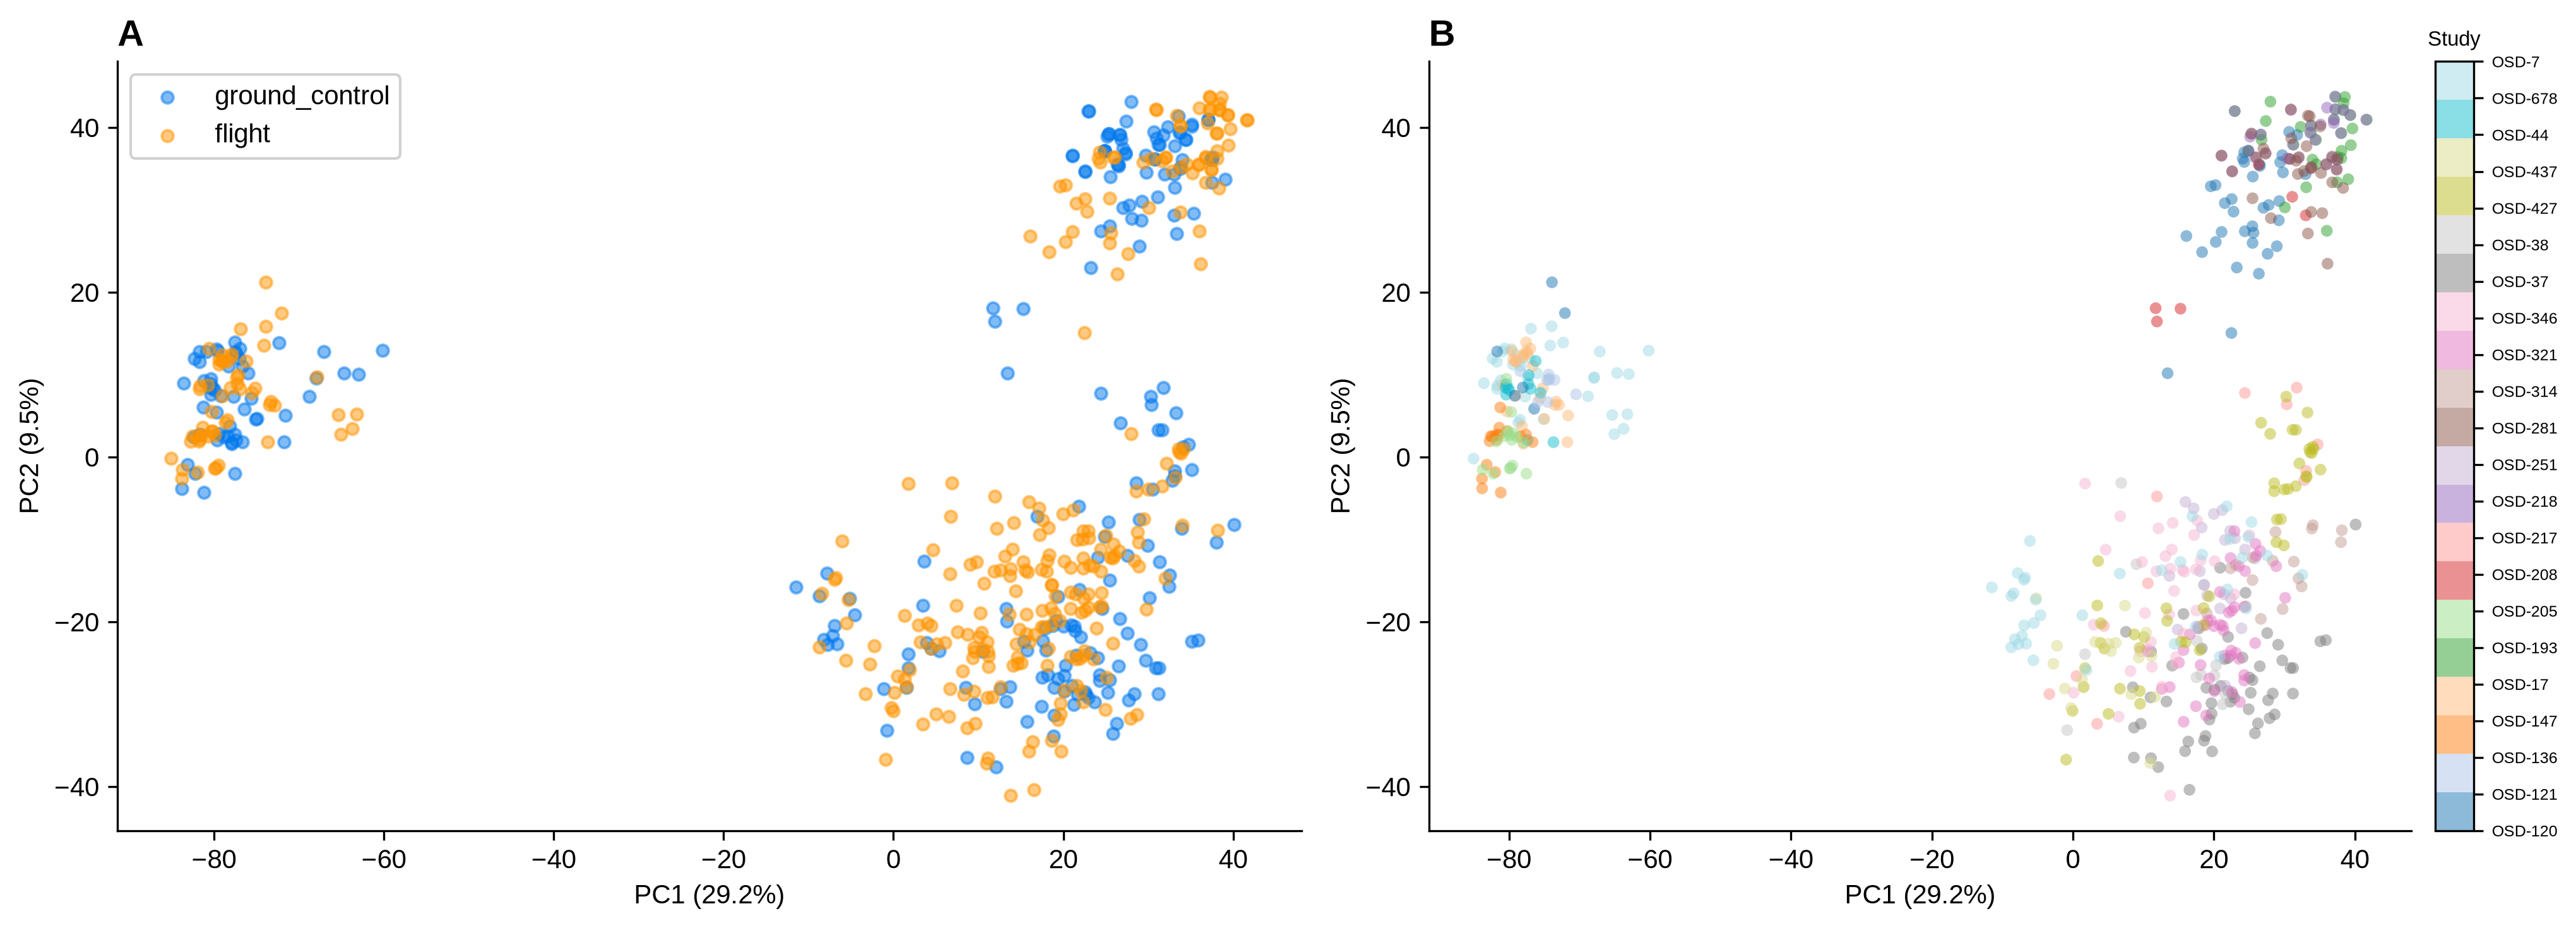
\includegraphics[width=0.9\textwidth]{figures/figS1_pca.png}
\caption{\textbf{Supplementary Figure S1. PCA of ChronoGauge sub-model predictions.} (\textbf{A}) PCA colored by condition (flight vs ground control). (\textbf{B}) PCA colored by study.}
\end{figure}

\begin{figure}[htbp]
\centering
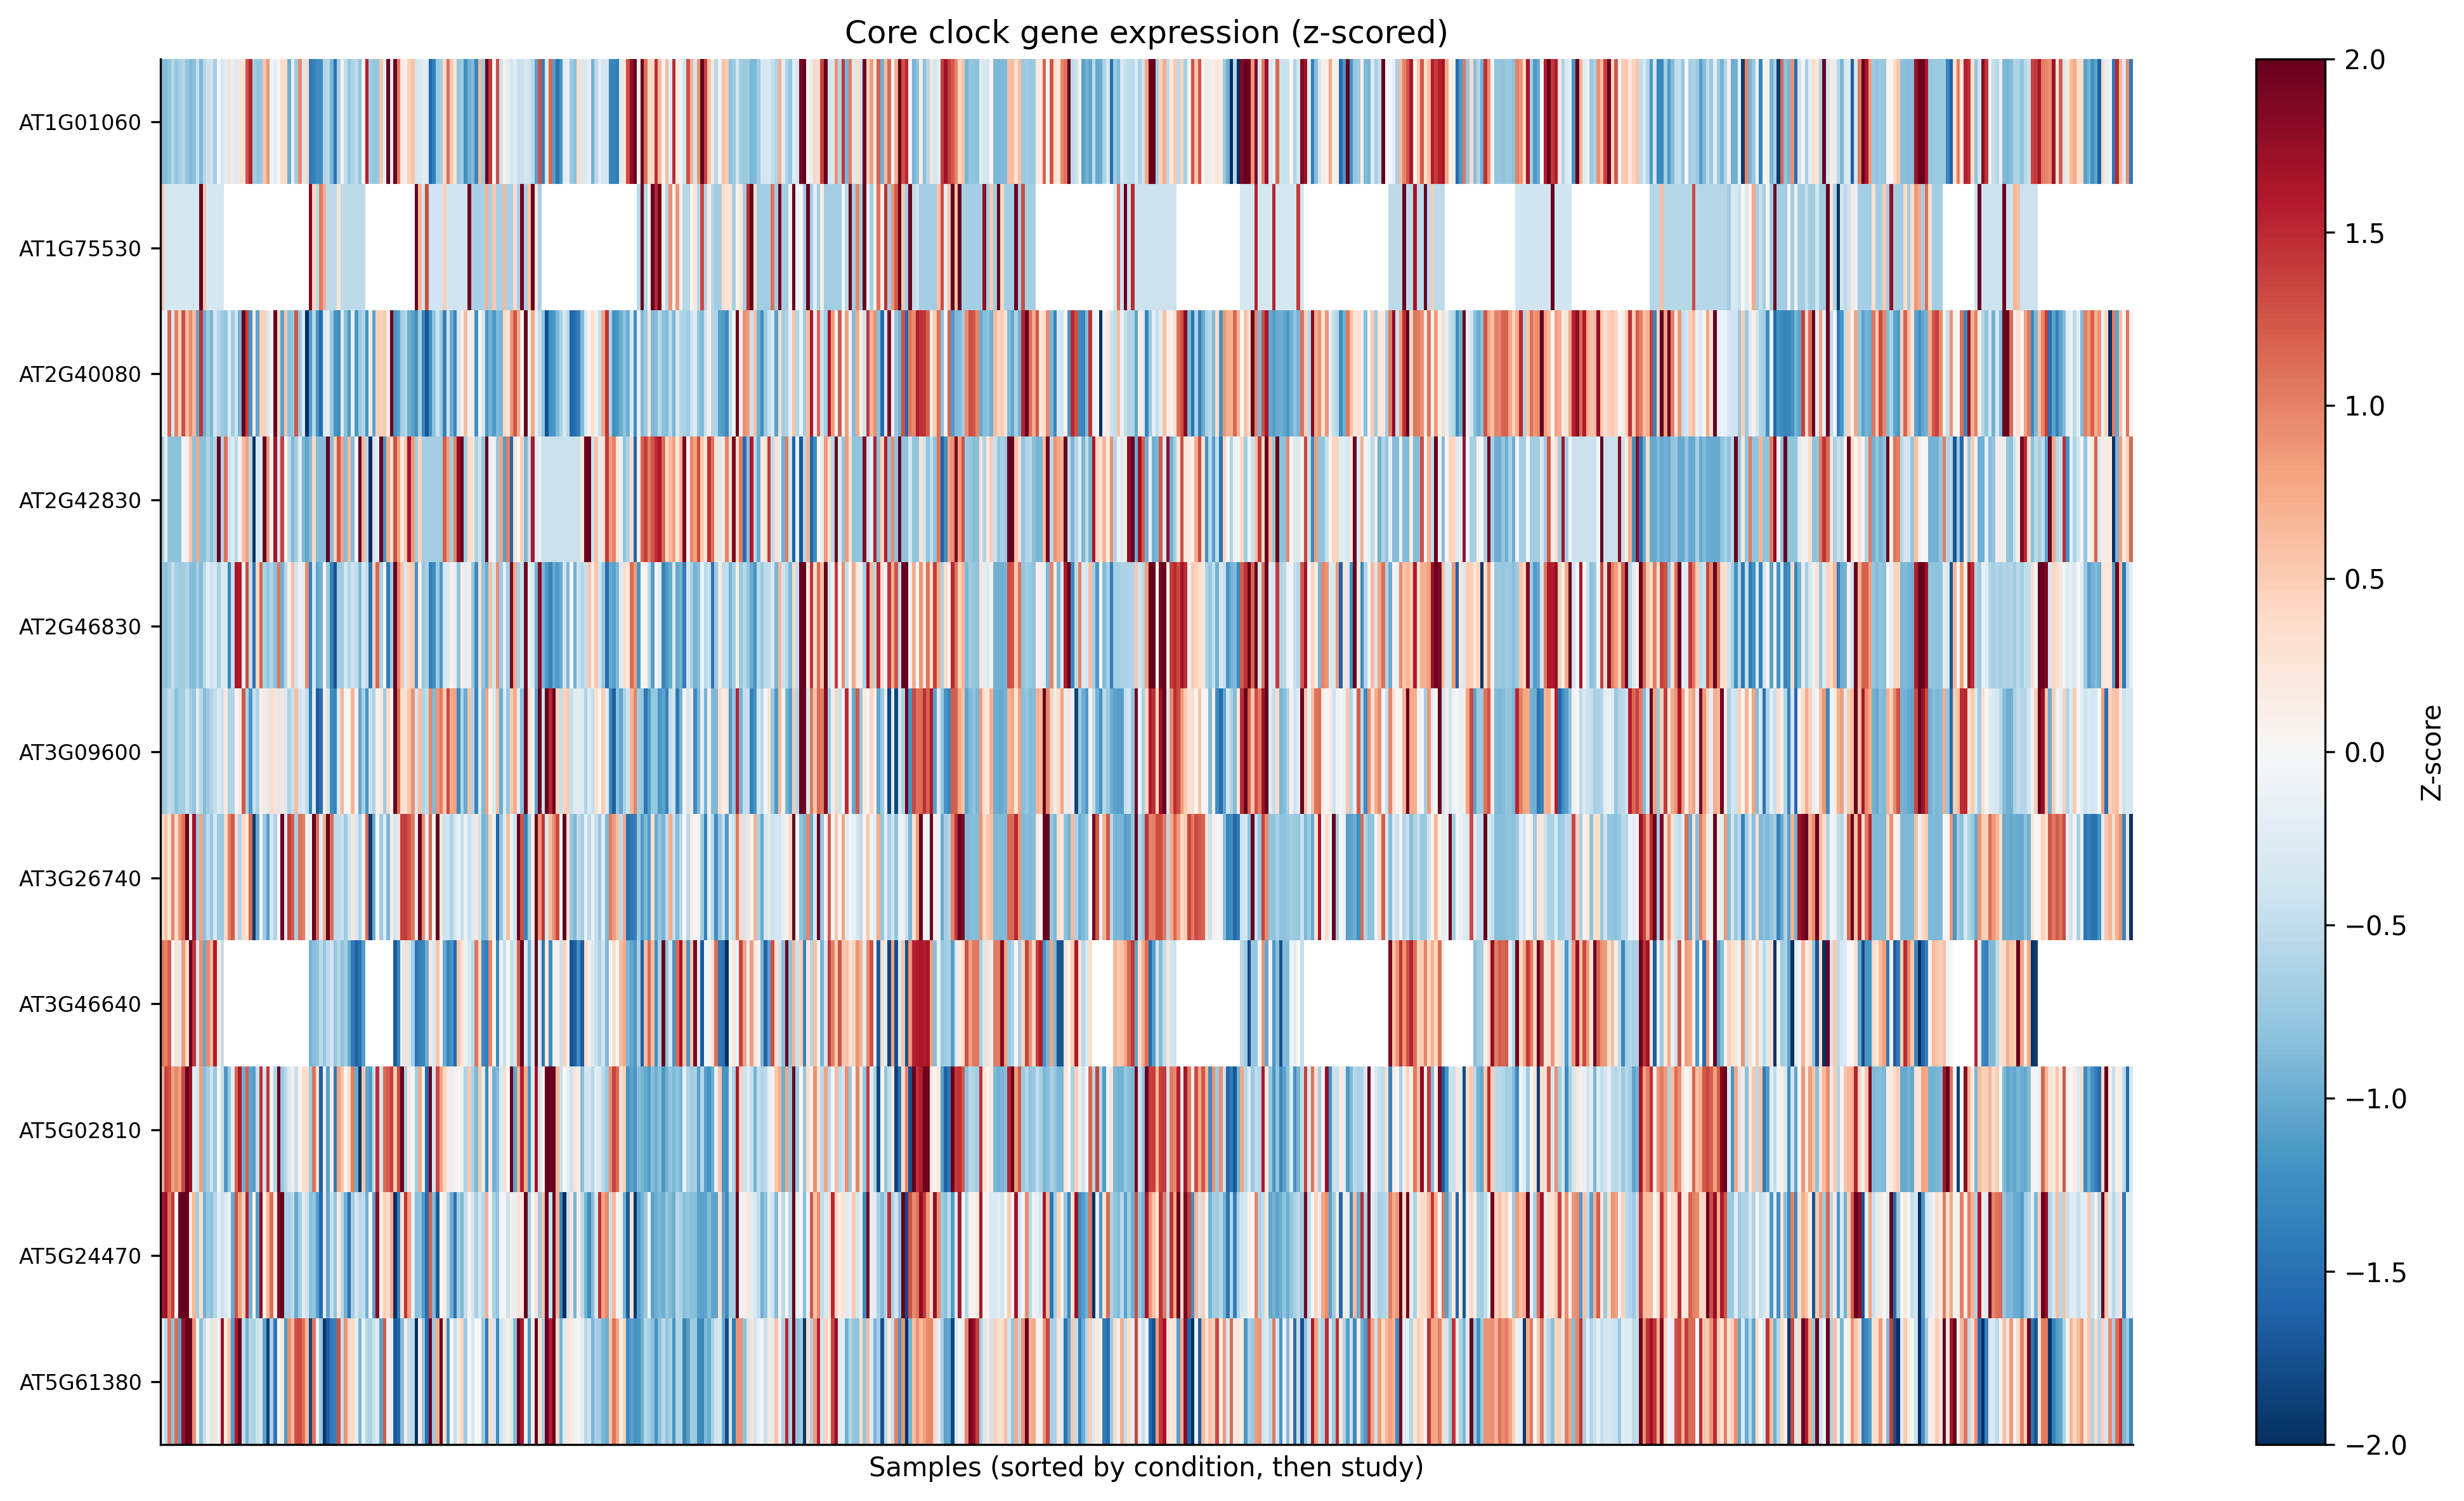
\includegraphics[width=0.9\textwidth]{figures/figS2_clock_genes.png}
\caption{\textbf{Supplementary Figure S2. Core clock gene expression heatmap.} Z-scored expression of core circadian clock genes (CCA1, LHY, TOC1, PRR9/7/5, GI, ELF4, ELF3, LUX, TIC) across all samples, sorted by condition and study.}
\end{figure}

\begin{figure}[htbp]
\centering
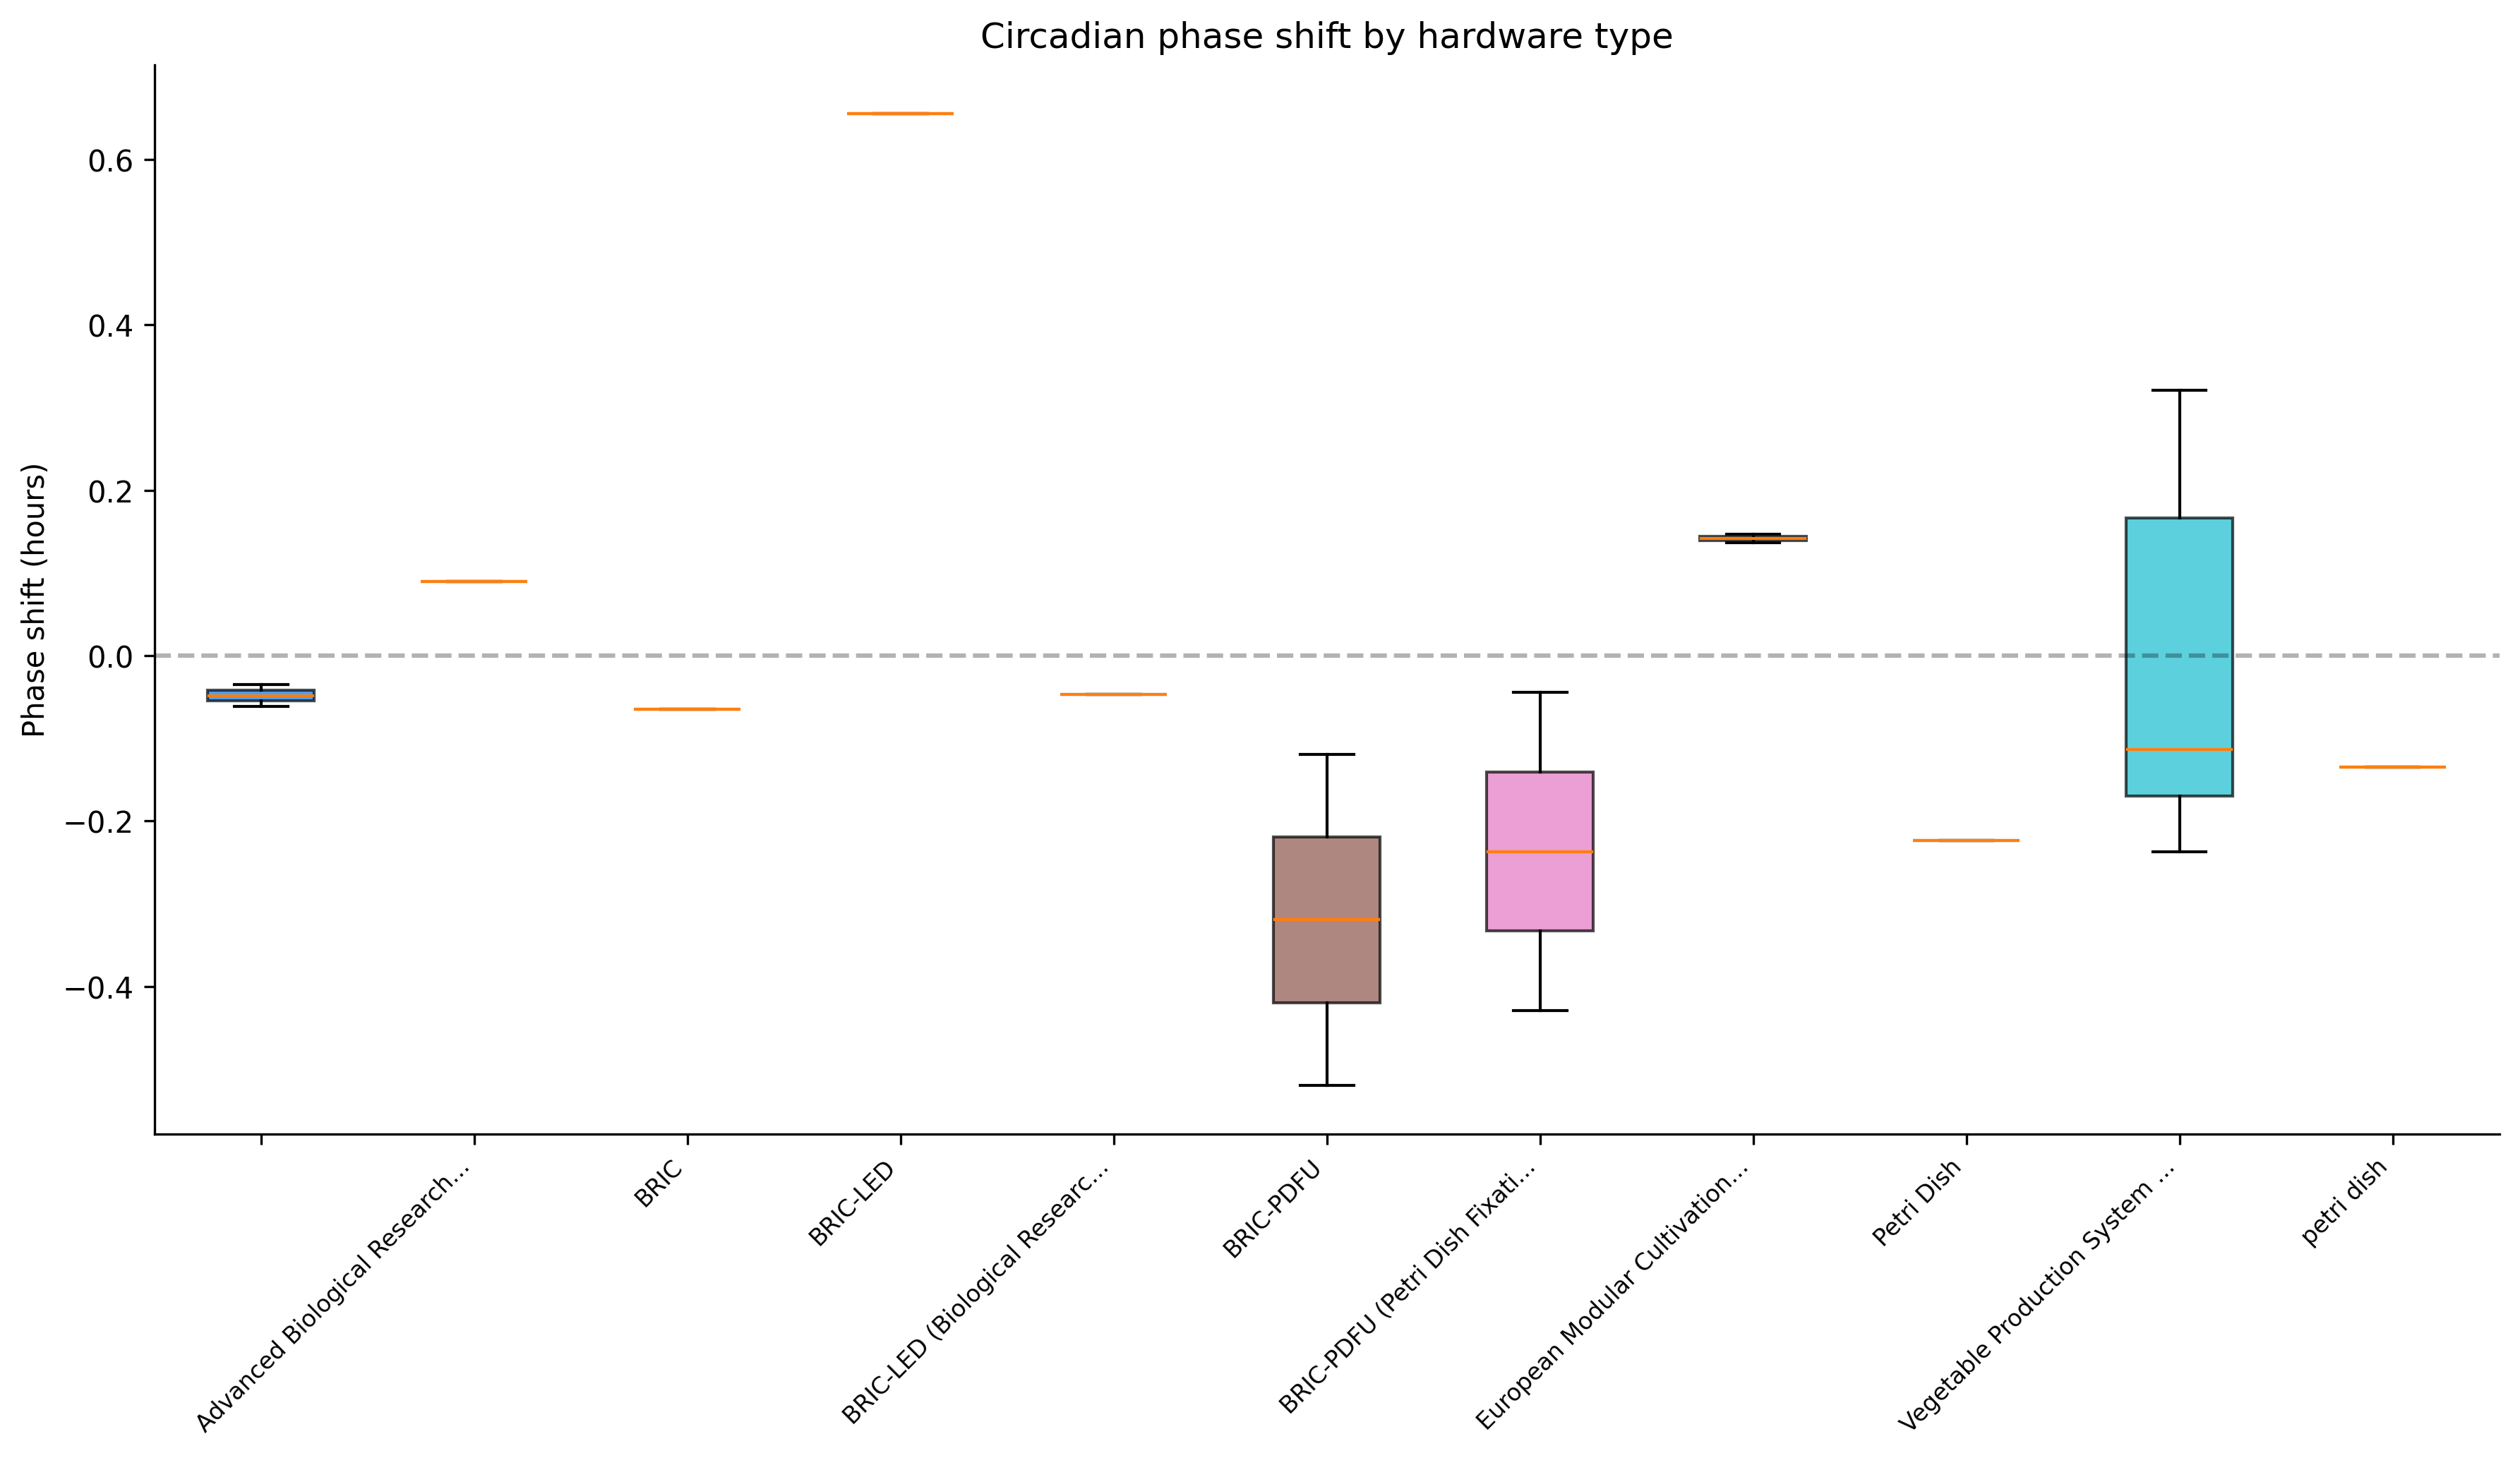
\includegraphics[width=0.8\textwidth]{figures/figS3_phase_by_hardware.png}
\caption{\textbf{Supplementary Figure S3. Phase shift by hardware type.} Box plots showing the distribution of per-study phase shifts grouped by hardware configuration.}
\end{figure}

\begin{figure}[htbp]
\centering
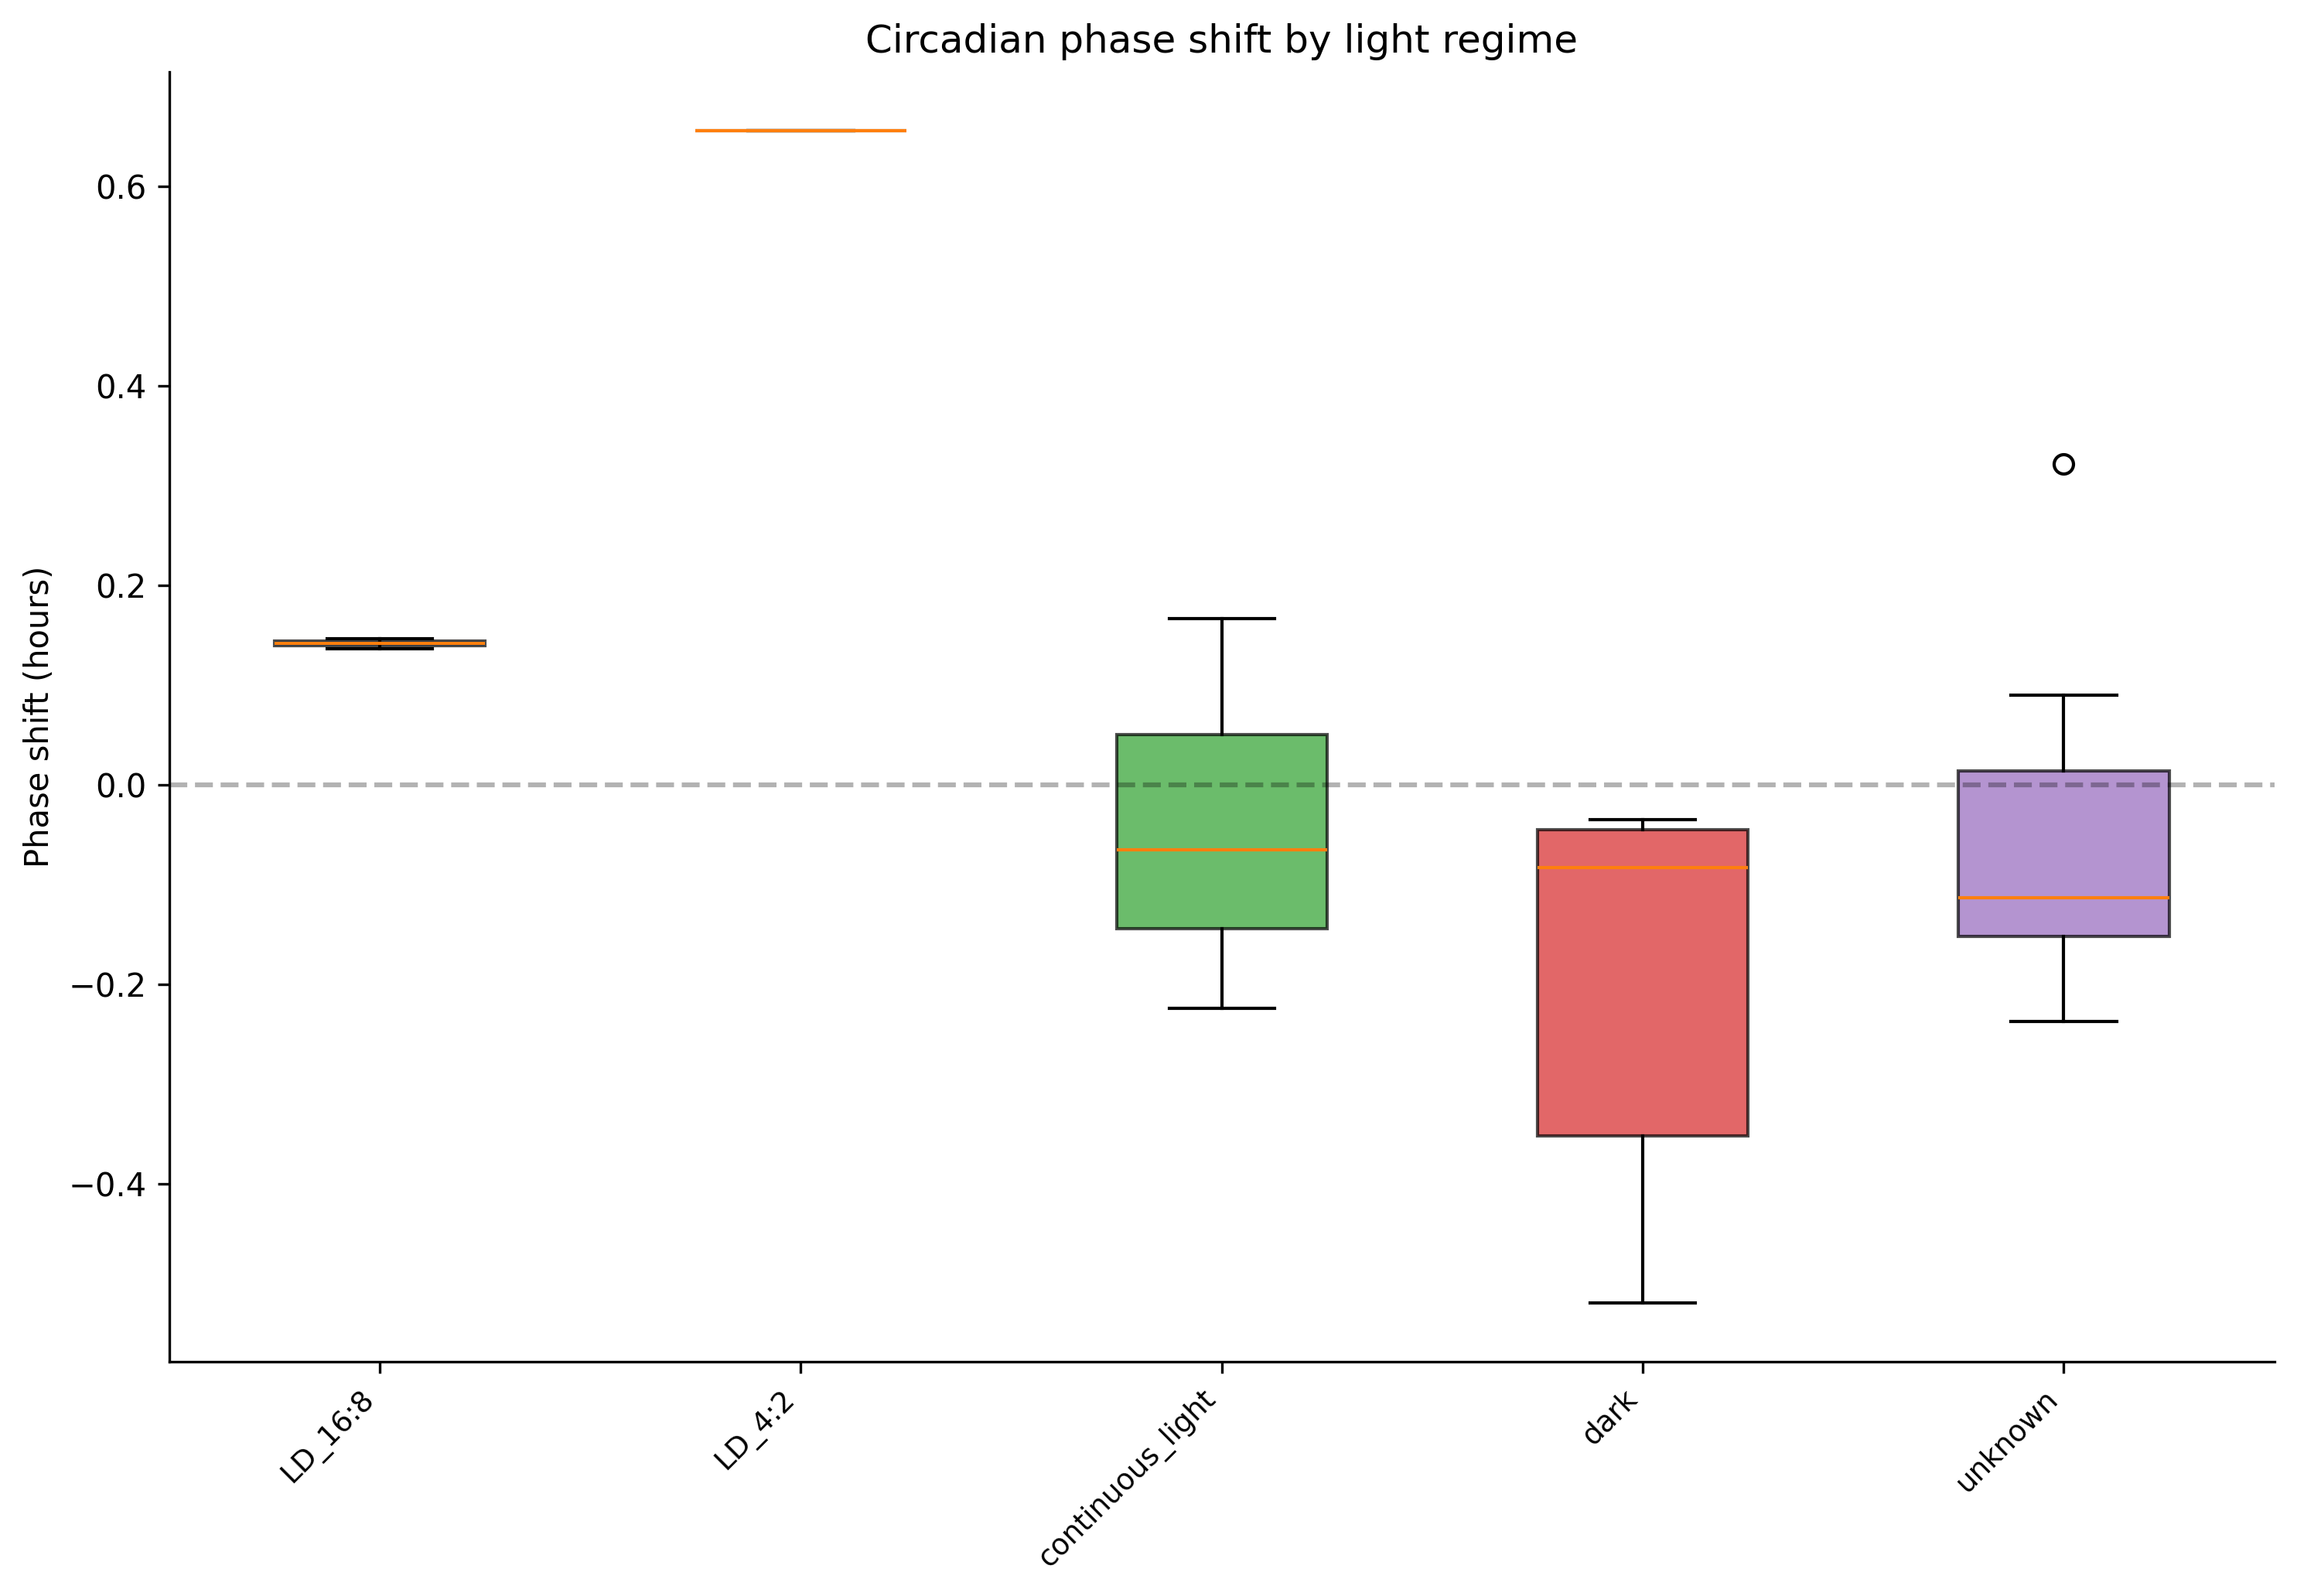
\includegraphics[width=0.8\textwidth]{figures/figS4_phase_by_light_regime.png}
\caption{\textbf{Supplementary Figure S4. Phase shift by light regime.} Box plots showing the distribution of per-study phase shifts grouped by light regime.}
\end{figure}

\begin{figure}[htbp]
\centering
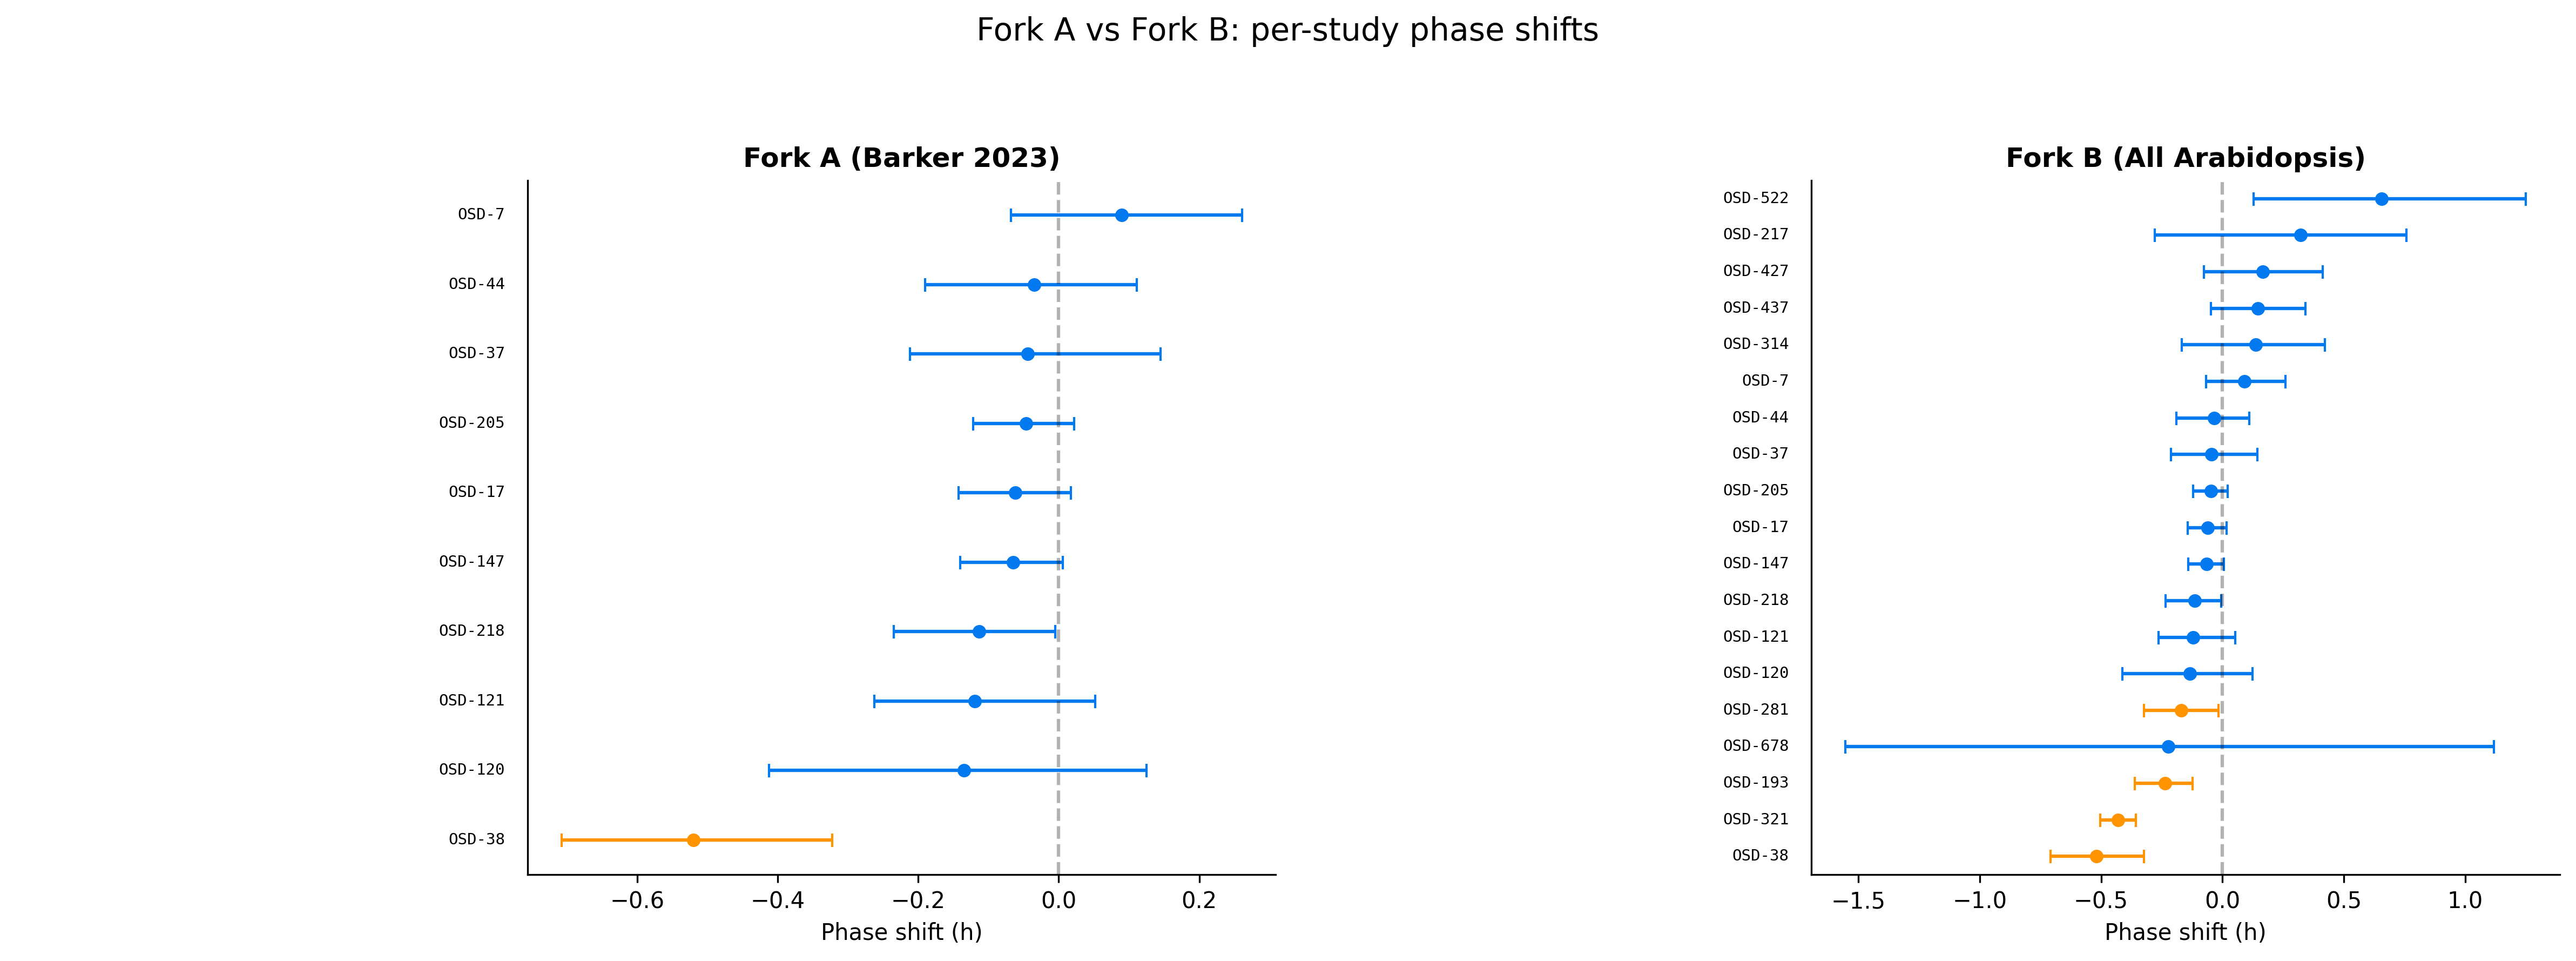
\includegraphics[width=\textwidth]{figures/figS5_fork_comparison.png}
\caption{\textbf{Supplementary Figure S5. Fork A versus Fork B comparison.} Per-study phase shifts for Fork A (Barker 2023 cohort, 14 studies) and Fork B (all Arabidopsis spaceflight transcriptomics, 24 studies).}
\end{figure}

\begin{figure}[htbp]
\centering
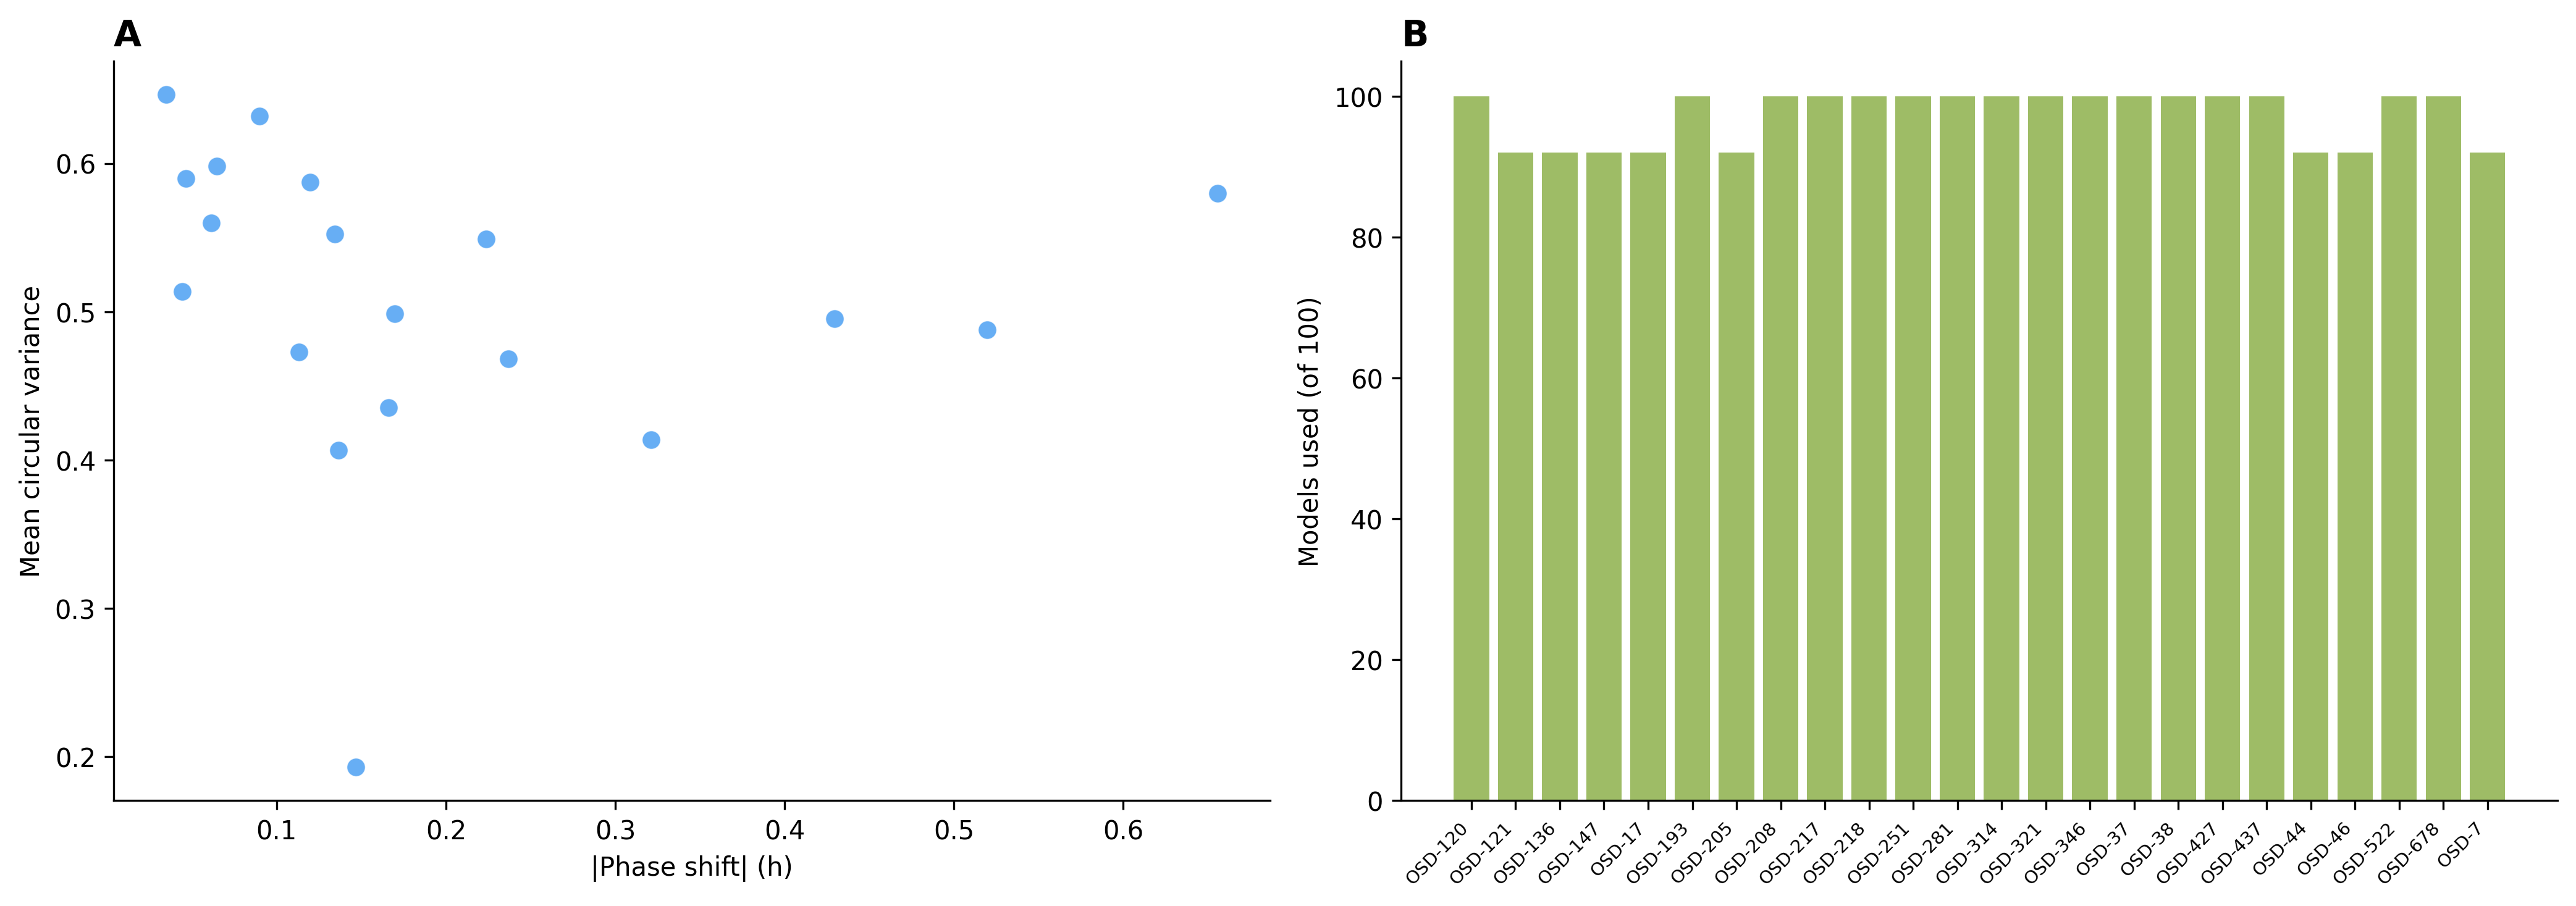
\includegraphics[width=0.9\textwidth]{figures/figS6_model_uncertainty.png}
\caption{\textbf{Supplementary Figure S6. Model uncertainty analysis.} (\textbf{A}) Relationship between phase shift magnitude and circular variance. (\textbf{B}) Number of ensemble sub-models used per study.}
\end{figure}

\section*{Supplementary Table}

\textbf{Supplementary Table S3.} Gene set enrichment results for the four studies with significant phase shifts (OSD-321, OSD-193, OSD-38, OSD-281). The table contains 2,459 pathway--study combinations with normalized enrichment scores (NES), $p$-values, FDR-adjusted $p$-values, and leading-edge genes for each gene set. Gene sets were derived from GO Biological Process terms and KEGG pathways via the \texttt{org.At.tair.db} annotation package (816 gene sets after filtering to 15--500 genes). The full table is provided as a CSV file (\texttt{tableS3\_enrichment\_results.csv}).

\section*{Data availability}

All data are publicly available from NASA GeneLab (\url{https://genelab.nasa.gov}). ChronoGauge pre-trained models are available from HuggingFace. Analysis code is available at [GitHub URL] and archived at [Zenodo DOI]. An interactive dashboard for exploring all results---including per-sample predictions, forest plots, circadian fingerprints, clock gene heatmaps, and t-SNE trajectories---is deployed at [GitHub Pages URL].

\section*{Code availability}

All analysis code is available at [GitHub URL] under the MIT license. A Docker container for reproducible analysis is available at [DockerHub URL].

\section*{Acknowledgements}

This research used data from NASA's GeneLab database. We thank the GeneLab team and all data contributors. We thank the ChronoGauge developers for making pre-trained models publicly available.

\section*{Author contributions}

R.B. conceived the study, designed the analysis, performed all computational work, and wrote the manuscript.

\section*{Competing interests}

The authors declare no competing interests.

\bibliographystyle{plainnat}

\begin{thebibliography}{15}
\bibitem[Covington et al.(2008)]{Covington2008} Covington, M.F., Maloof, J.N., Straume, M., Kay, S.A. \& Harmer, S.L. Genome-wide analysis of the \textit{Arabidopsis} clock reveals complex regulation. \textit{Genome Biology} 9, R167 (2008).
\bibitem[Harmer et al.(2000)]{Harmer2000} Harmer, S.L. et al. Orchestrated transcription of key pathways in \textit{Arabidopsis} by the circadian clock. \textit{Science} 290, 2110--2113 (2000).
\bibitem[Pokhilko et al.(2012)]{Pokhilko2012} Pokhilko, A., Fern\'andez, A.P., Edwards, K.D., Southern, M.M., Halliday, K.J. \& Millar, A.J. The clock gene circuit in \textit{Arabidopsis} includes a repressilator with additional feedback loops. \textit{Molecular Systems Biology} 8, 574 (2012).
\bibitem[Dodd et al.(2005)]{Dodd2005} Dodd, A.N., Salathia, N., Hall, A., K\'evei, E., T\'oth, R., Nagy, F., Hibberd, J.M., Millar, A.J. \& Webb, A.A.R. Plant circadian clocks increase photosynthesis, growth, survival, and competitive advantage. \textit{Science} 309, 630--633 (2005).
\bibitem[Paul et al.(2012)]{Paul2012} Paul, A.L., Amalfitano, C.E. \& Ferl, R.J. Plant growth strategies are remodeled by spaceflight. \textit{BMC Plant Biology} 12, 232 (2012).
\bibitem[Nayak et al.(2020)]{Nayak2020} Nayak, K.K. et al. Spaceflight-induced changes in the Arabidopsis circadian clock. \textit{npj Microgravity} 6, 21 (2020).
\bibitem[Kiss et al.(2019)]{Kiss2019} Kiss, J.Z., Kumar, P., Millar, K.D.L., Edelmann, R.E. \& Correll, M.J. Operations of a spaceflight experiment to study plant tropisms. \textit{Gravitational and Space Research} 7, 1--14 (2019).
\bibitem[Barker et al.(2023)]{Barker2023} Barker, R. et al. A meta-analysis of \textit{Arabidopsis thaliana} spaceflight transcriptome data. \textit{npj Microgravity} 9, 23 (2023).
\bibitem[Hughes et al.(2010)]{Hughes2010} Hughes, M.E., Hogenesch, J.B. \& Kornacker, K. JTK\_CYCLE: an efficient nonparametric algorithm for detecting rhythmic components in genome-scale data. \textit{Journal of Biological Rhythms} 25, 372--380 (2010).
\bibitem[Thaben \& Westermark(2014)]{Thaben2014} Thaben, P.F. \& Westermark, P.O. Detecting rhythms in time series with RAIN. \textit{Journal of Biological Rhythms} 29, 391--400 (2014).
\bibitem[Reynolds et al.(2025)]{Reynolds2025} Reynolds, W. et al. ChronoGauge: a deep learning approach for circadian time prediction from single transcriptomic samples. \textit{bioRxiv} 2025.01.12.573912 (2025).
\bibitem[Watson \& Williams(1956)]{Watson1956} Watson, G.S. \& Williams, E.J. On the construction of significance tests on the circle and the sphere. \textit{Biometrika} 43, 344--352 (1956).
\bibitem[DerSimonian \& Laird(1986)]{DerSimonian1986} DerSimonian, R. \& Laird, N. Meta-analysis in clinical trials. \textit{Controlled Clinical Trials} 7, 177--188 (1986).
\bibitem[Viechtbauer(2010)]{Viechtbauer2010} Viechtbauer, W. Conducting meta-analyses in R with the metafor package. \textit{Journal of Statistical Software} 36, 1--48 (2010).
\bibitem[Mancuso et al.(2019)]{Mancuso2019} Mancuso, S., Barlow, P.W., Volkmann, D. \& Balu\v{s}ka, F. Gravity as a morphogenetic factor in plants. \textit{Journal of Plant Growth Regulation} 38, 1--12 (2019).
\bibitem[Rakusov\'a et al.(2011)]{Rakusova2011} Rakusov\'a, H., Gallego-Bartolom\'e, J., Vanstraelen, M., Robert, H.S., Alabad\'i, D. \& Friml, J. Polarization of PIN3-dependent auxin transport for hypocotyl gravitropic response in \textit{Arabidopsis thaliana}. \textit{The Plant Journal} 67, 817--826 (2011).
\bibitem[Ritchie et al.(2015)]{Ritchie2015} Ritchie, M.E., Phipson, B., Wu, D., Hu, Y., Law, C.W., Shi, W. \& Smyth, G.K. limma powers differential expression analyses for RNA-sequencing and microarray studies. \textit{Nucleic Acids Research} 43, e47 (2015).
\bibitem[Korotkevich et al.(2021)]{Korotkevich2021} Korotkevich, G., Sukhov, V., Budin, N., Shpak, B., Artyomov, M.N. \& Sergushichev, A. Fast gene set enrichment analysis. \textit{bioRxiv} 2021.06.15.448424 (2021).
\end{thebibliography}

\end{document}
